\section{Desarrollo}

Una vez pasada a la fase de desarrollo, el objetivo es transformar el diseño y requisitos concretados previamente en una aplicación funcional. 

Este proceso implica la creación de la skill, el desarrollo de código y la realización de pruebas, pero no sin antes haber cumplido dos prerrequisitos:
\begin{itemize}
	\item Tener una cuenta en \textit{Alexa developer console}, que es de carácter totalmente gratuito y permitirá el alojamiento y despliegue de la skill. 
	\item Tener una cuenta de \textit{Amazon Web Services} (AWS), para lo que se debe ingresar un método de pago. Esto es necesario en caso de que el uso de recursos exceda los límites de la oferta gratuita y Amazon tenga que cobrar una cantidad adicional.
\end{itemize}

\subsection{Creación de la skill y el modelo de interacción}

Hay una gran cantidad de guías disponibles para aprender a crear una skill desde cero, y la propia página oficial de desarrolladores Alexa \parencite{alexaHosted} ofrece diversos documentos de apoyo, los cuales se han utilizado como material de referencia en esta etapa del proyecto.

\begin{enumerate}
	\item Una vez iniciada la sesión en la consola de desarrolladores de Alexa, se abre el menú de creación de skills.
	\item Se elige la región donde se van a alojar los servicios AWS predeterminados de la nueva skill, en este caso, la opción \textit{eu-west-1}, localizada en Irlanda, que es la más cercana.
	\item Se selecciona un nombre para la skill y el idioma para el que va a estar implementado el modelo.
	\item Para la decisión del modelo, el que mejor se ajusta a las especificaciones de este proyecto es el \textit{Custom model} (o personalizado), que permite una mayor flexibilidad.
	\item Como la idea es que Alexa se encargue de alojar el backend de la skill, se elige una de las dos opciones de \textit{Alexa-hosted}, en este caso la del entorno de ejecución de Node.js v16.x.
	\item Se puede añadir una plantilla o importar una skill alojada en un repositorio de Git. En este caso, se ha optado por trabajar a partir de una plantilla básica, que solo incluye un ejemplo simple de \enquote{\textit{Hello world}} (ver figura 29). Sobre esta base se añadirán todas las funcionalidades del juego.
\end{enumerate}

\begin{figure}[H]
	\centering
	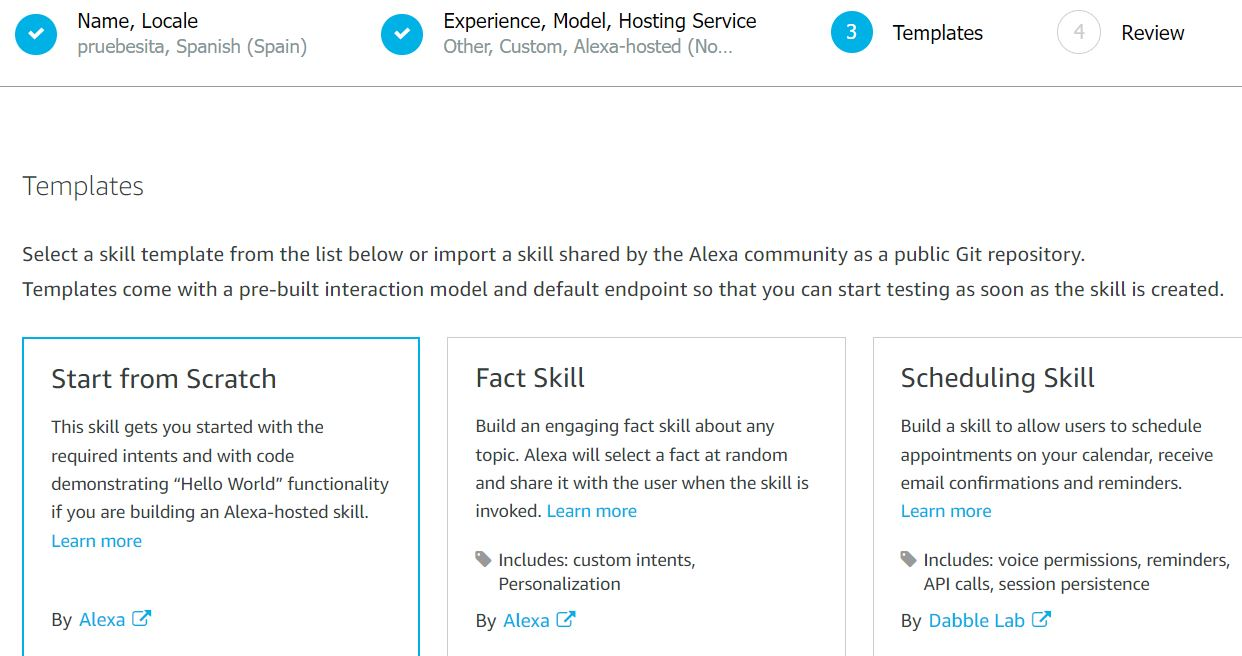
\includegraphics[width=1\textwidth]{imgs/alexa-dev-console-2.jpg}
	\caption{Menú de creación de una skill de Alexa}
	\label{fig:alexa-dev-console-2}
\end{figure}

Una vez creada y finalizada la configuración básica, se abrirá automáticamente el menú de \textit{Build}, desde el que se pueden ajustar varios aspectos de la skill.

Lo primero es declarar el nombre de invocación, que es con el que se llamará a la función de lanzamiento en el momento en el que se abre la skill, y se puede ajustar desde el menú lateral de \textit{Invocations}. Alexa establece una serie de restricciones sobre este parámetro: no puede incluir artículos o preposiciones, debe componerse de mínimo dos palabras, si contiene números estos deben ser escritos de manera completa, no debe incluir mayúsculas ni palabras reservadas como \enquote{Alexa, skill, app,} etc. 

El nombre de invocación elegido es \enquote{probando oca}, por tanto cuando se quiera iniciar la skill, habrá que decir: \enquote{Alexa, abre probando oca}.

Otro elemento desplegable revelante del menú lateral es el modelo de interacción (\textit{Interaction Model}), donde se definen los \textit{intents}. Inicialmente hay cinco predeterminados, de los cuales cuatro son de carácter obligatorio y por tanto no pueden borrarse:

\begin{itemize}
	\item \textbf{AMAZON.CancelIntent}: cancela la acción actual y termina la interacción con la skill.
	\item \textbf{AMAZON.HelpIntent}: proporciona información sobre cómo usar la habilidad.
	\item \textbf{AMAZON.StopIntent}: detiene la acción en curso y finaliza la interacción con la skill.
	\item \textbf{AMAZON.NavigateHomeIntent}: regresa al inicio de o a la pantalla principal.
	\item \textbf{HelloWorldIntent}: ejecuta la acción personalizada predefinida, que consiste en saludar a la persona usuaria. Es la única que puede eliminarse.
\end{itemize}

También se puede acceder y modificar el archivo JSON del modelo de interacción directamente, aunque es aconsejable utilizar en lugar de ello la interfaz de configuración, ya que cada vez que se monta la skill este fichero se actualiza automáticamente.

Otro elemento interesante son los Assets, que permiten la creación de tipos personalizados de slots, la consulta del historial de compilación de la skill y la configuración del \textit{endpoint}. 

Al tratarse de una skill alojada por Alexa, el endpoint se trata de la función Lambda de AWS encargada de la ejecución del código de la skill. Además, por defecto se dispone de tres de ellos, localizados en distintas regiones del mundo: Virginia del Norte, Irlanda y Oregon.

\begin{figure}[H]
	\centering
	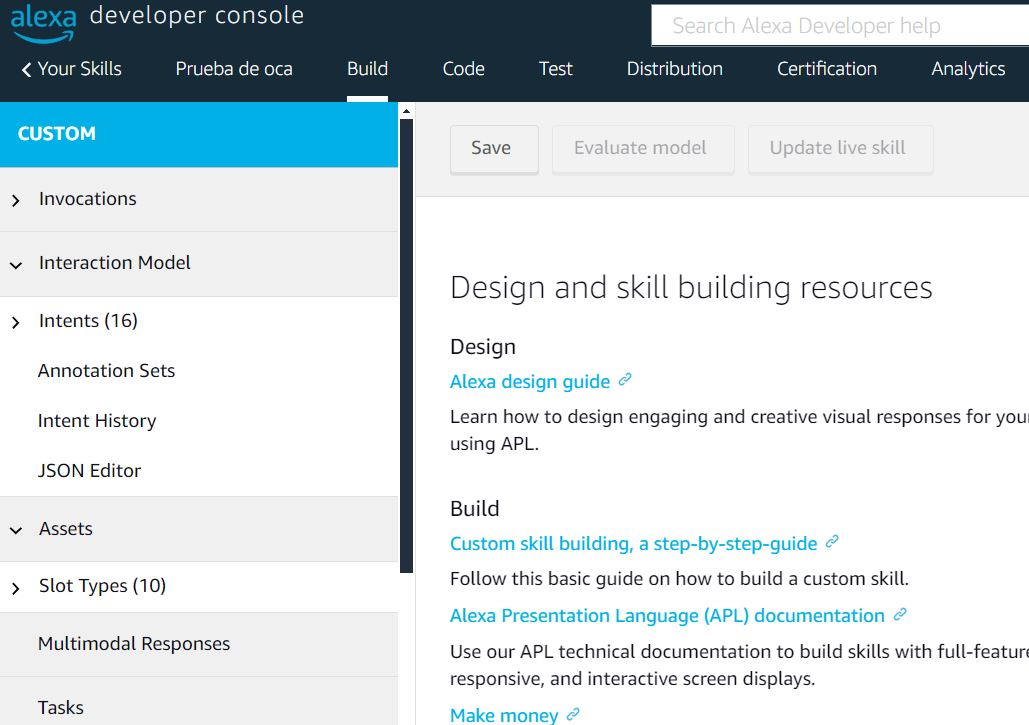
\includegraphics[width=1\textwidth]{imgs/alexa-dev-console-1.jpg}
	\caption{Menú principal de montaje de la skill de Alexa}
	\label{fig:alexa-dev-console-1}
\end{figure}

Si se navega al menú de código desde la barra de herramientas, se puede encontrar la siguiente estructura de archivos:

\begin{figure}[H]
	\centering
	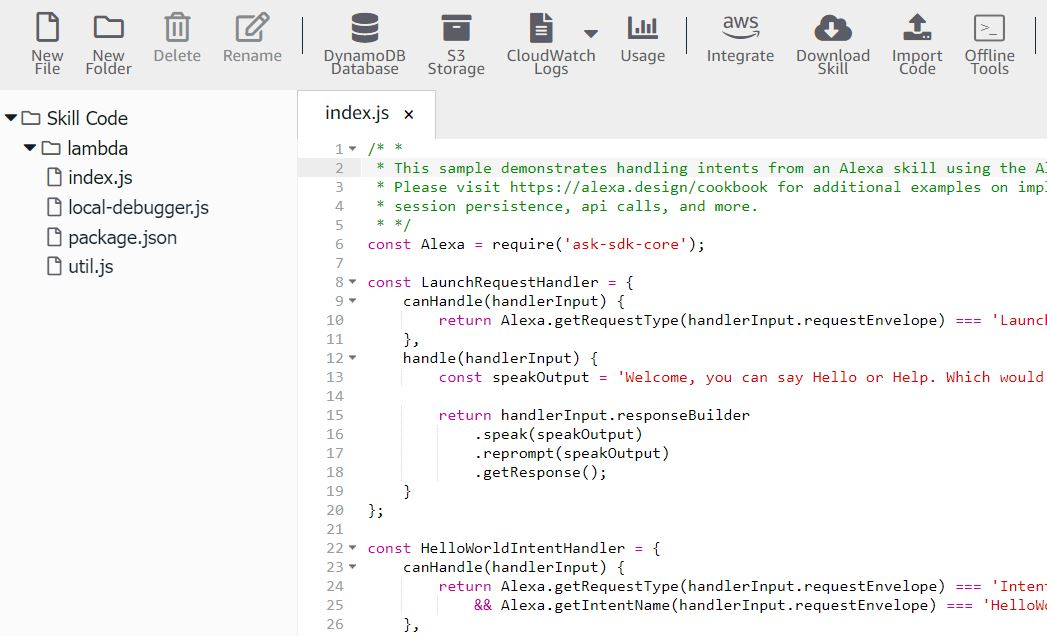
\includegraphics[width=1\textwidth]{imgs/alexa-dev-console-3.jpg}
	\caption{Menú del código de la skill de Alexa}
	\label{fig:alexa-dev-console-3}
\end{figure}

El fichero \textit{index.js} es el más importante, ya que actúa como entrypoint o punto de entrada de la skill, donde se exporta la función de Lambda. Es el que gestiona todos los handlers (manejadores de solicitudes), que determinan el flujo de conversación de Alexa gracias a la capacidad de establecer respuestas concretas a cada intent. Los handlers predefinidos son:
\begin{itemize}
	\item \textbf{LaunchRequestHandler}:  se activa cuando se abre la skill sin especificar un comando, respondiendo con un mensaje de bienvenida.
	\item \textbf{HelloWorldIntentHandler}: responde cuando el usuario invoca a \textit{HelloWorldIntent}, que se limita a saludar.
	\item \textbf{HelpIntentHandler}: maneja el \textit{AMAZON.HelpIntent}, puede invocarse cuando se necesita ayuda.
	\item \textbf{CancelAndStopIntentHandler}: gestiona \textit{AMAZON.CancelIntent} y \textit{AMAZON.StopIntent}, que sirve para detener la skill.
	\item \textbf{FallbackIntentHandler}: se activa se dice algo que no coincide con ninguno de los intents definidos.
	\item \textbf{SessionEndedRequestHandler}: se invoca cuando una sesión termina, ya sea por un comando de usuario o error.
	\item \textbf{IntentReflectorHandler}: útil para la depuración de la skill, ya que responde con el nombre del intent con el que fue llamado. 
	\item \textbf{ErrorHandler}: sirve para la captura de errores de cualquier tipo.
\end{itemize}

Otro archivo esencial en cualquier proyecto realizado con Node.js es \textit{package.json}, donde se definen las dependencias y bibliotecas requeridas, además de permitir la configuración de scripts, pruebas e información acerca de la versión, nombre del proyecto, etc.

Por otro lado, los dos ficheros restantes (\textit{local-debugger.js} y \textit{util.js}) no han sido necesarios para el desarrollo del proyecto, pero pueden servir como base para facilitar la depuración local de la skill y definir funciones de utilidad generales.

\subsection{Configuración de servicios de AWS}

La plataforma de servicios AWS ofrece una amplia gama de mecanismos de monitorización, almacenamiento, gestión de políticas, computación, etc. Se caracteriza, entre otras cosas, por la flexibilidad y escalabilidad que permite gracias a su modelo de \enquote{pagar solo lo que se usa}.

En la consola de desarrolladores de AWS aparecen todos los servicios usados recientemente, facilitando la navegación entre ellos.

\begin{figure}[H]
	\centering
	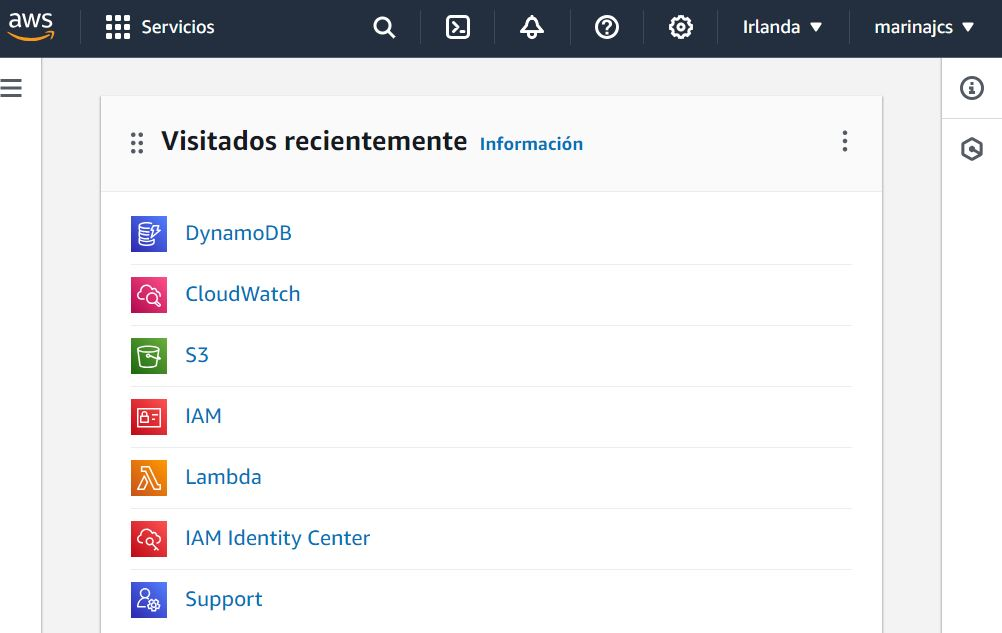
\includegraphics[width=0.7\textwidth]{imgs/aws-console-1.jpg}
	\caption{Menú de la consola de desarrolladores de AWS}
	\label{fig:aws-console-1}
\end{figure}


\subsubsection{Identity and Access Management (IAM)}

El primer servicio utilizado es IAM, con el objetivo de crear un rol capaz de otorgar permisos temporales de acceso a DynamoDB a skills de Alexa.

\begin{figure}[H]
	\centering
	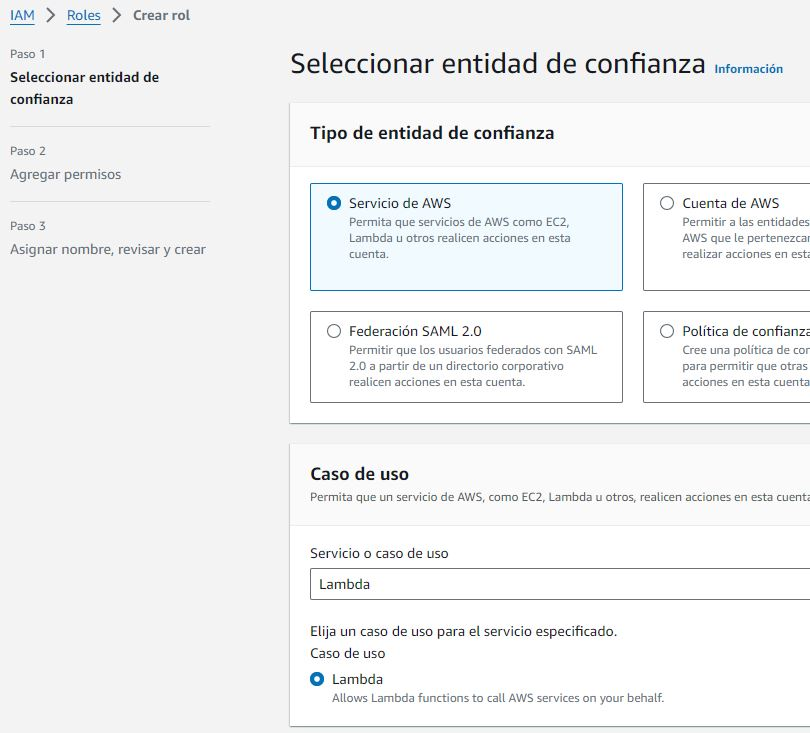
\includegraphics[width=1\textwidth]{imgs/aws-iam-2.jpg}
	\caption{Menú de creación de un rol IAM}
	\label{fig:aws-iam-2}
\end{figure}

En el menú de creación del rol, hay que rellenar los siguientes parámetros de configuración: el tipo de entidad de confianza (un servicio de AWS), el caso de uso (la función de Lambda), las políticas de permisos a agregar (\textit{AmazonDynamoDBFullAccess}) y el nombre del rol que se está creando.

\begin{figure}[H]
	\centering
	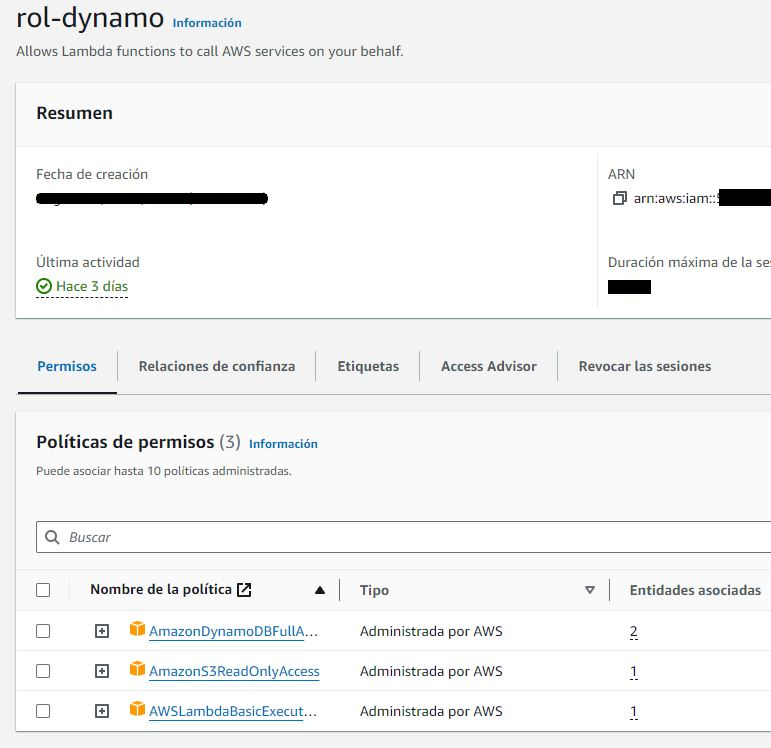
\includegraphics[width=1\textwidth]{imgs/aws-iam-1.png}
	\caption{Rol creado para la skill y sus permisos en AWS}
	\label{fig:aws-iam-1}
\end{figure}

Para que la skill pueda usar los recursos de AWS que será definidos en las secciones siguientes, se necesita modificar el fichero JSON que especifica las relaciones de confianza del rol. Para ello, se añade la siguiente entrada:

\begin{figure}[H]
	\centering
	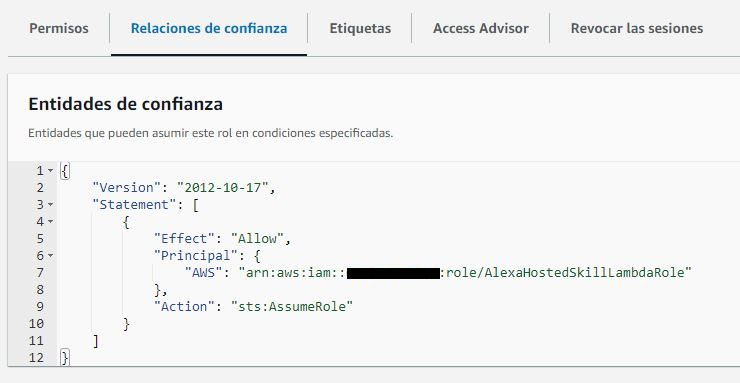
\includegraphics[width=1\textwidth]{imgs/aws-iam-3.png}
	\caption{Configuración de las relaciones de confianza del rol}
	\label{fig:aws-iam-3}
\end{figure}

El texto censurado es el ARN (Amazon Resource Name) o identificador del rol de ejecución IAM que la función Lambda asume al ejecutarse la skill de Alexa. Este se puede obtener desde la consola de desarrolladores de Alexa, en el menú del código, con la opción \textit{Integrate}, especialmente diseñada para poder vincular la skill a servicios personales de AWS.

\begin{figure}[H]
	\centering
	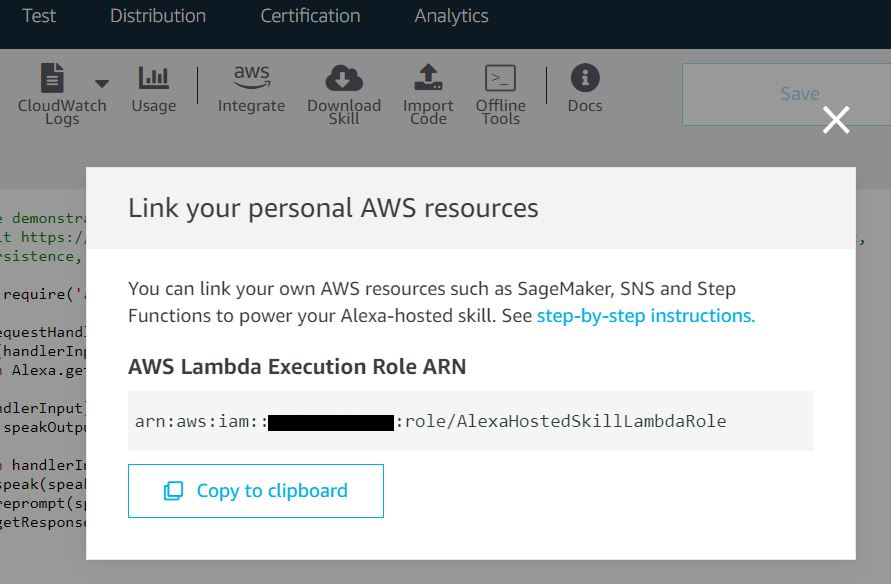
\includegraphics[width=0.75\textwidth]{imgs/aws-iam-4.png}
	\caption{El AWS Lambda Execution Role ARN de la skill}
	\label{fig:aws-iam-4}
\end{figure}

\subsubsection{Amazon Simple Storage Service (S3)}

Como su nombre indica, es un servicio ofrecido en AWS que permite almacenar objetos de diversos tipos (textos, binarios, documentos, audios, comprimidos, etc). Sin embargo, dados los requisitos de este juego, solo será necesario guardar lo siguiente: las imágenes asociadas a cada casilla, la de la pantalla de bienvenida y los vídeos con las animaciones de los lanzamientos de dado.

En Amazon S3, se ha adoptado el término de \textit{bucket} como un contenedor para almacenar objetos. Cada bucket tiene un nombre único y puede simular una estructura de directorios, además pueden ser de acceso público o privado, al igual que sus elementos, que pueden configurarse a través de políticas de acceso.

Para este proyecto, se ha creado un bucket de nombre \textit{bucket-oca} para guardar todos los archivos multimedia que necesita la skill.

\begin{figure}[H]
	\centering
	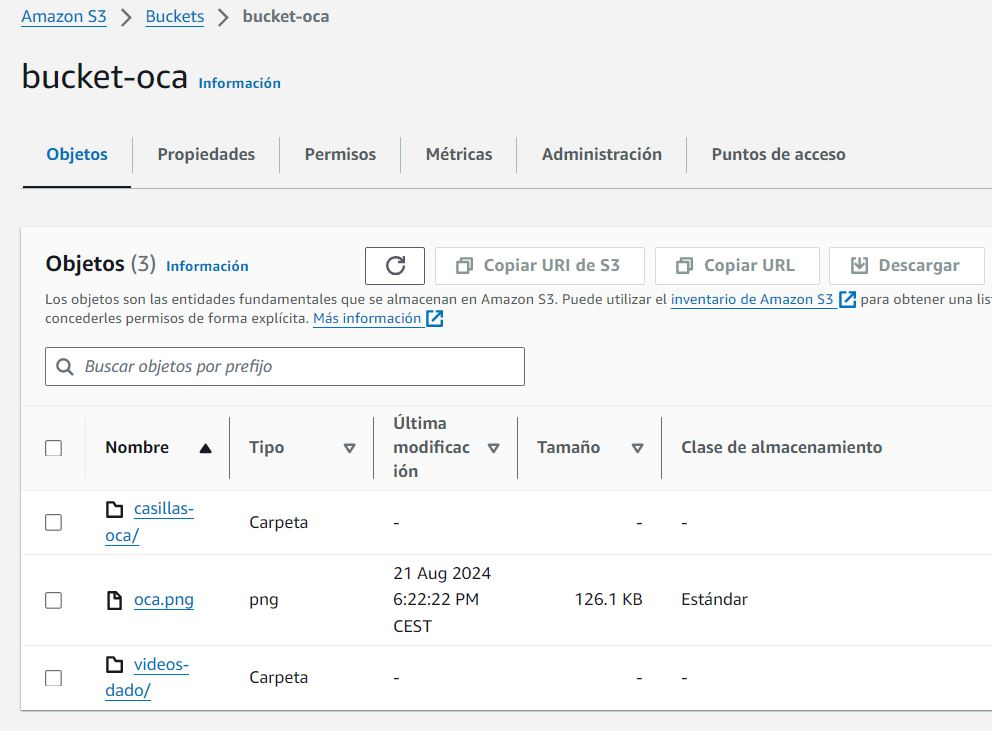
\includegraphics[width=1\textwidth]{imgs/aws-s3-1.jpg}
	\caption{Bucket de Amazon S3 para la skill de la oca}
	\label{fig:aws-s3-1}
\end{figure}

\subsubsection{DynamoDB}

Como se ha mencionado en la sección \textit{6.1.2.}, los datos de una skill no persisten de una sesión a otra, por lo que es necesario un mecanismo para guardarlos. Aquí entra el papel de las bases de datos, en particular DynamoDB, también intergado en AWS.

Esta base de datos es de tipo NoSQL y es una alternativa interesante no solo por su total compatibilidad con las herramientas actuales del proyecto debido a que es otro servicio Amazon, sino también por su alta capacidad de adaptación a cualquier volumen de datos. 

Es conocido por optimizar sus tiempos de respuesta y llevar a cabo un escalado automático en función del tráfico, gracias a su esquema NoSQL, cuyos elementos de las tablas se identifican mediante claves primarias únicas. Estas últimas pueden ser de partición o compuestas (unión de una clave de partición con una de ordenamiento). Para este proyecto, se han creado dos tablas: 
\begin{itemize}
	\item \textbf{JuegoOca}: su clave primaria es \textit{idJuego}, que siempre valdrá 0 debido a que se pretende guardar los datos de una sola partida entre sesiones. Tiene los elementos generales de un juego de la oca, que son el estado, el turno y ronda actual, el número de jugadores, el tipo de participantes...
	\item \textbf{Jugador}: identificada por la clave primaria \textit{idJugador}, que a la vez determina el orden de turno, y será un valor entero único entre 0 y el el numero de total de participantes menos uno. Los atributos de cada elemento son: el nombre, el color, los puntos, la posición y penalizaciones actuales, etc.
\end{itemize} 

\begin{figure}[H]
	\centering
	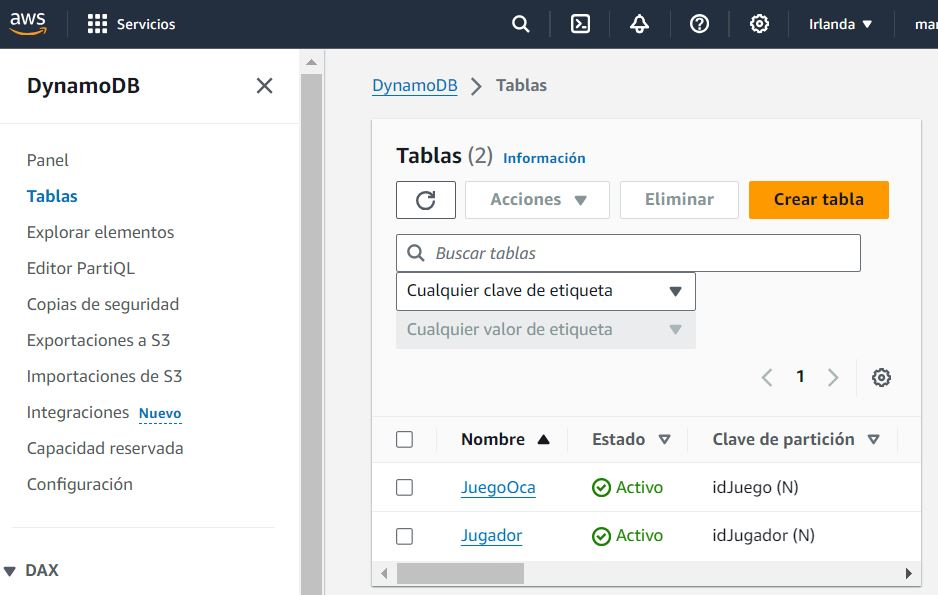
\includegraphics[width=0.8\textwidth]{imgs/aws-db-1.jpg}
	\caption{Tablas \textit{JuegoOca} y \textit{Jugador} creadas en DynamoDB}
	\label{fig:aws-db-1}
\end{figure}

Desde la consola de AWS, dentro del servicio de DynamoDB, se pueden explorar los elementos guardados en las tablas, así como consultar las unidades de lectura/escritura consumidas hasta el momento.

\begin{figure}[H]
	\centering
	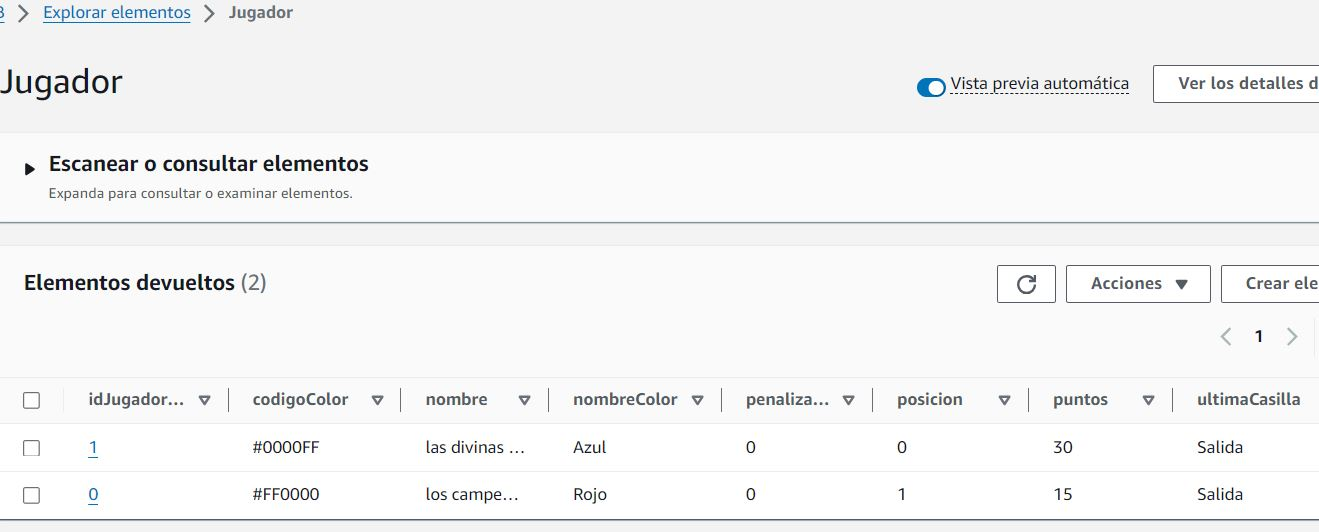
\includegraphics[width=1\textwidth]{imgs/aws-db-2.jpg}
	\caption{Información de la tabla \textit{Jugador} de DynamoDB}
	\label{fig:aws-db-2}
\end{figure}

\subsection{Implementación y estructura del código}

La estructura de archivos del código de la función de Lambda que ejecuta la skill del juego es la siguiente:

\begin{figure}[H]
	\centering
	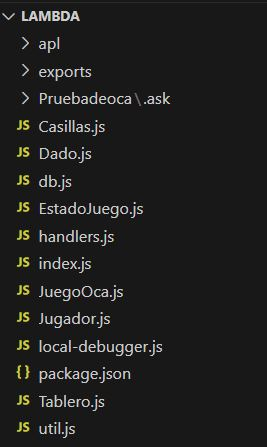
\includegraphics[width=0.3\textwidth]{imgs/estructura-codigo.jpg}
	\caption{Estructura del código de la función Lambda}
	\label{fig:estructura-codigo}
\end{figure}

A continuación se explicarán los contenidos de los ficheros, salvo: \textit{local-debugger.js}, \textit{package.json} y \textit{util.js}, que ya fueron descritos en la sección \textit{7.1.}

\subsubsection{Lógica del juego de la oca}

Consiste en la implementación de las clases definidas en el modelo conceptual de la sección \textit{5.3}, que cubren las funcionalidades del juego de la oca.

\paragraph{Fichero \enquote{Jugador.js}}

Define la clase encargada de representar a cada participante, ya sea un equipo o jugador/a individual, que va a competir en el juego de la oca.

\begin{figure}[H]
	\centering
	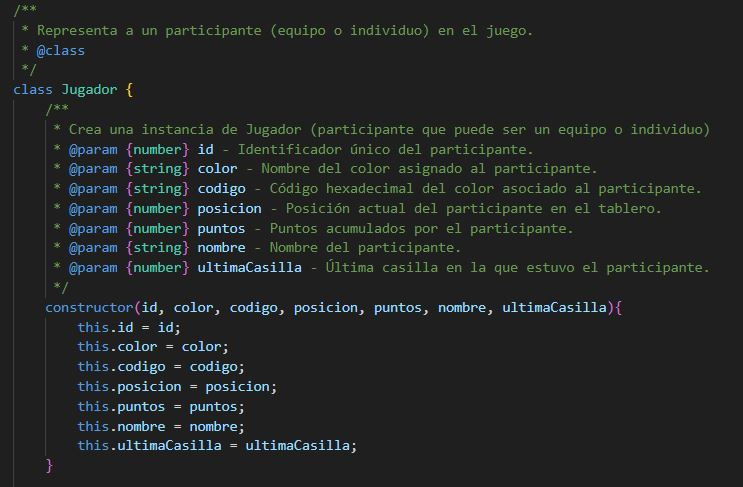
\includegraphics[width=0.8\textwidth]{imgs/codigo-jugador.jpg}
	\caption{Clase jugador junto con su constructor}
	\label{fig:codigo-jugador}
\end{figure}

También incluye \textit{setters} y \textit{getters} para poder modificar y consultar cada atributo de clase.

\paragraph{Fichero \enquote{Dado.js}}

Está constituido por dos funciones auxiliares: la primera, que realiza un lanzamiento de dado, devolviendo un número aleatorio entre 1 y 6, y la segunda, para obtener la dirección URL del vídeo asociado a cada resultado posible de una tirada. Esto será especialmente útil cuando se vaya a implementar el APL más adelante.

\begin{figure}[H]
	\centering
	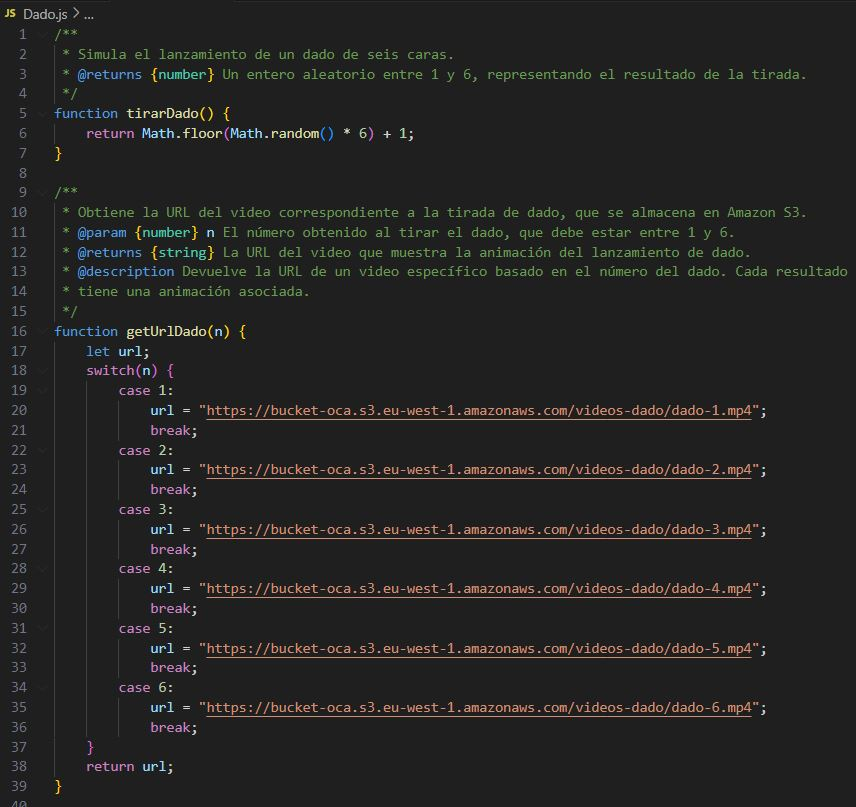
\includegraphics{imgs/codigo-dado.jpg}
	\caption{Funciones que componen el módulo del dado}
	\label{fig:codigo-dado}
\end{figure}

\paragraph{Fichero \enquote{Casillas.js}}

En las primeras líneas se realizan las importaciones necesarias de los datos de las preguntas que se usarán para los minijuegos, así como las frases de carácter descriptivo que se invocarán cuando se caiga en cualquier casilla.

\begin{figure}[H]
	\centering
	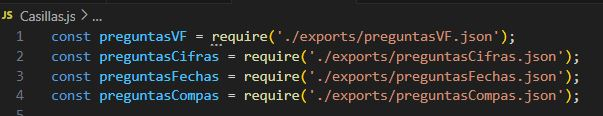
\includegraphics[width=0.8\textwidth]{imgs/codigo-casillas-1.jpg}
	\caption{Importaciones de las baterías de preguntas de los minijuegos}
	\label{fig:codigo-casillas-1}
\end{figure}

\newpage
Luego, se define la clase que representa una casilla general (o de carácter normal); es decir, aquella que no desencadena ningún evento especial como desplazarse a otra casilla, tirar el dado de nuevo, iniciar un minijuego, etc.

\begin{figure}[H]
	\centering
	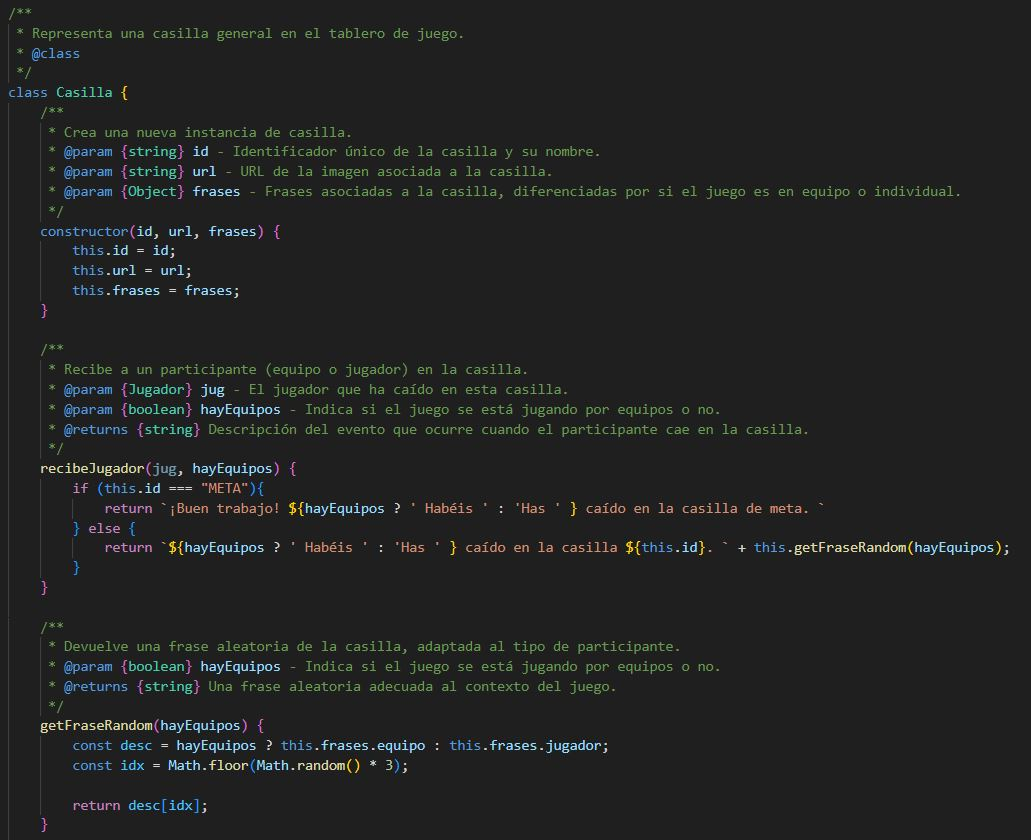
\includegraphics[width=1\textwidth]{imgs/codigo-casillas-2.jpg}
	\caption{Declaración de la clase de una casilla normal}
	\label{fig:codigo-casillas-2}
\end{figure}

Se puede ver cómo hay dos métodos: \textit{getFraseRandom()}, encargado de devolver una descripción aleatoria de la casilla normal, habiendo tres posibles opciones para cada una, y \textit{recibeJugador()}, que informa al participante sobre dónde ha caído, incluyendo la descripción de la misma. 
Este último método será sobrescrito en las distintas clases que heredan de \textit{Casilla}, para adaptar los informes en función del tipo de la instancia. Por ejemplo, si es una casilla de oca, dirá \enquote{de oca en oca y tiro porque me toca}, si es una de minijuego, anunciará qué tipo de pregunta hará y cómo jugar, etc.

\subparagraph{Casillas especiales tradicionales: oca, puente y penalización}

Siguiendo el esquema del juego de mesa tradicional, las casillas de oca permiten moverse a la siguiente del mismo y tirar el dado de nuevo; las casillas de puente, transportan a la otra casilla del mismo tipo independientemente de si dicho movimiento supone un avance o retroceso en el tablero; y las casillas de penalización, como la del pozo y el laberinto, hacen perder turnos a cualquiera que caiga en ellas.

Las casillas de oca y de puente mantienen una estructura similar a su superclase, con los mismos atributos y la única diferencia en el método sobrescrito de \textit{recibeJugador()}; sin embargo, la clase \textit{CasillaPenalizacion} incluye un nuevo atributo (\textit{penaliza}) que representa el número de turnos que deben pasar antes de poder avanzar de nuevo.

\begin{figure}[H]
	\centering
	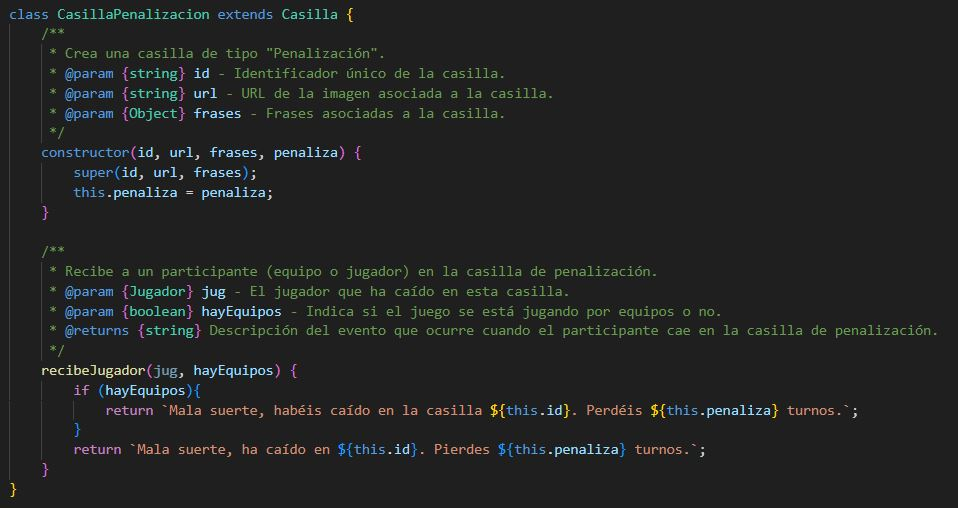
\includegraphics{imgs/codigo-casillas-3.jpg}
	\caption{Declaración de la clase de casillas de penalización}
	\label{fig:codigo-casillas-3}
\end{figure}

\subparagraph{Casillas de minijuegos personalizadas}

Se caracterizan porque además de los métodos heredados de las casillas normales, cuentan con un método llamado \textit{getPreguntaRandom()}, que devuelve un elemento aleatorio de la batería de preguntas del tipo correspondiente, con la excepción del minijuego de \enquote{recuerda la última casilla}, que no necesita el método porque la pregunta siempre es la misma.

Por tanto, la clase que define la casilla del minijuego de verdadero o falso tendría la siguiente apariencia:

\begin{figure}[H]
	\centering
	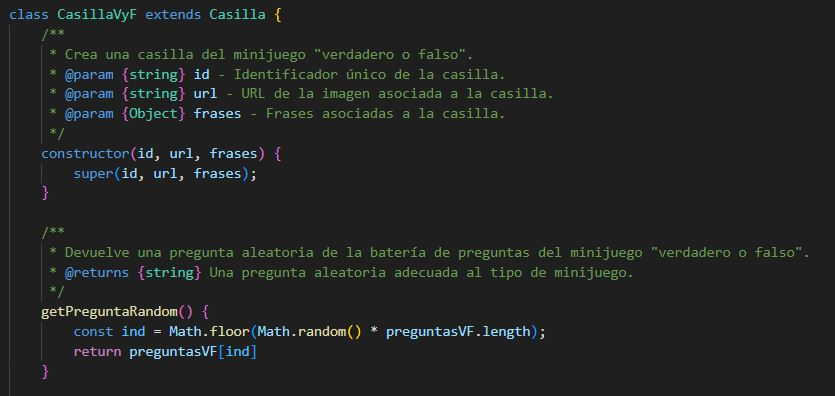
\includegraphics{imgs/codigo-casillas-4.jpg}
	\caption{Clase para casilla del minijuego verdadero o falso}
	\label{fig:codigo-casillas-4}
\end{figure}

En el minijuego de \enquote{conoce a tus compañeros} también se necesita guardar el nombre del equipo/participante sobre el que va la pregunta, así que sehace una ligera modificación, pasándole como argumento un arreglo con todos los compañeros del jugador o jugadora actual.

\begin{figure}[H]
	\centering
	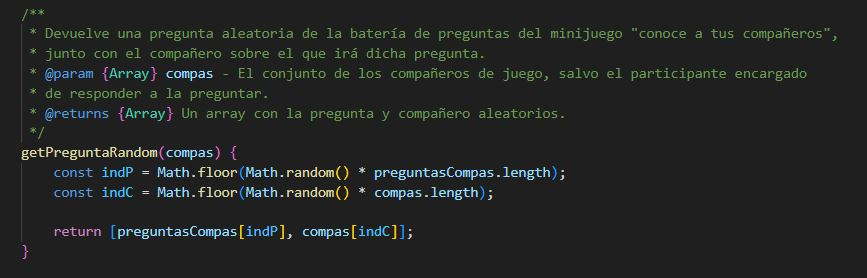
\includegraphics{imgs/codigo-casillas-5.jpg}
	\caption{Método para obtener una pregunta aleatoria sobre un compañero}
	\label{fig:codigo-casillas-5}
\end{figure}

Las clase para la casilla del minijuego \enquote{adivina la cifra} es parecida a la de la figura 44. Por otro lado, como en el minijuego de \enquote{recuerda la fecha} se manejan tres tipos distintos de preguntas y respuestas (día de la semana, mes o estación del año), y la solución correcta se calcula a partir de la fecha actual, o lo que es lo mismo, no es un valor estático, entonces requiere añadir una serie de métodos adicionales:

\begin{figure}[H]
	\centering
	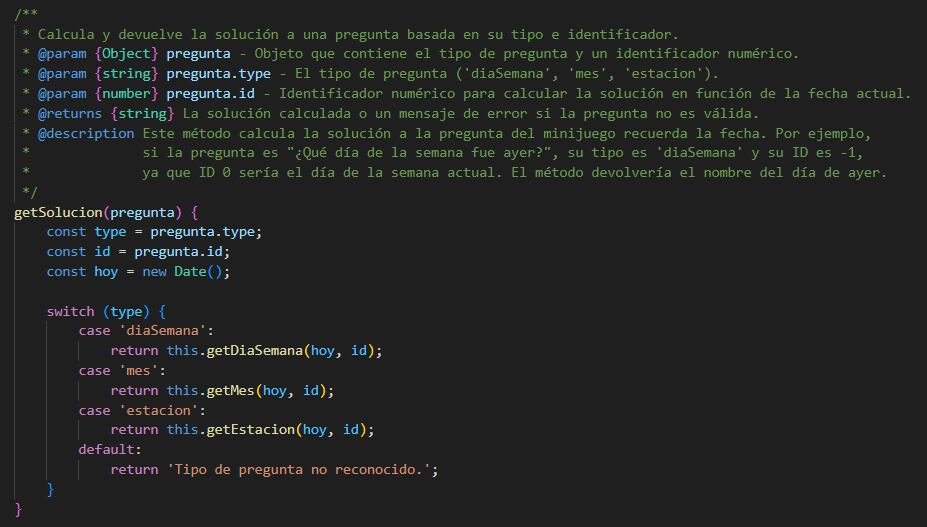
\includegraphics{imgs/codigo-casillas-6.jpg}
	\caption{Método para obtener la solución de una pregunta de fecha}
	\label{fig:codigo-casillas-6}
\end{figure}

En la figura anterior, aparecen invocaciones a tres métodos auxiliares que permiten el cálculo correcto de la respuesta pasándole como argumentos el valor de la fecha actual y un id o número de desplazamiento partiendo del actual. Si el id es igual a 0, entonces la solución es el día/mes/estación actual; si el id es 1, la respuesta es el día/mes/estación siguiente al actual; si el id es -1, el anterior al actual... Y así sucesivamente. 

\begin{figure}[H]
	\centering
	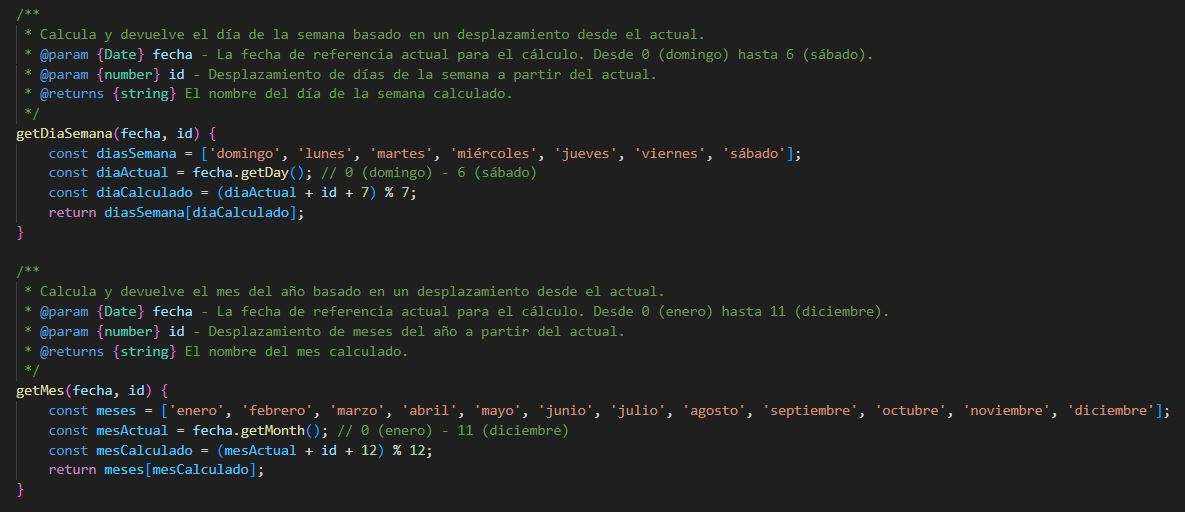
\includegraphics[width=1\textwidth]{imgs/codigo-casillas-7.jpg}
	\caption{Cálculo de días de la semana o meses a partir de la fecha actual}
	\label{fig:codigo-casillas-7}
\end{figure}

\begin{figure}[H]
	\centering
	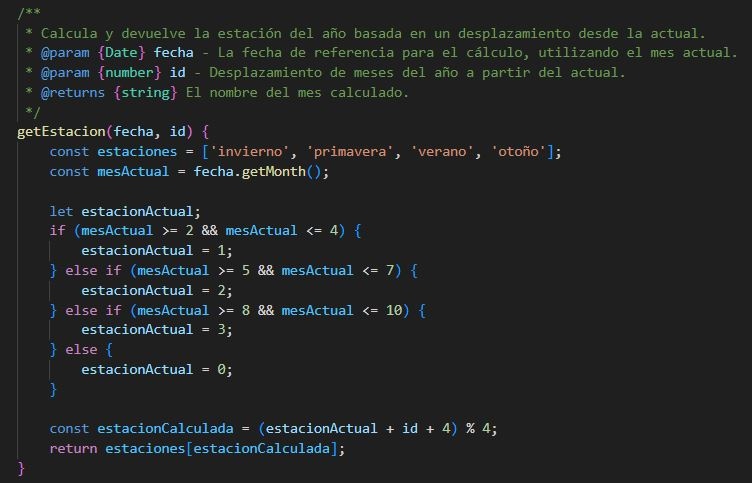
\includegraphics[width=0.82\textwidth]{imgs/codigo-casillas-8.jpg}
	\caption{Cálculo de la estación del año partiendo de la fecha actual}
	\label{fig:codigo-casillas-8}
\end{figure}

\paragraph{Fichero \enquote{Tablero.js}}

Es la estructura que almacena todas las casillas del juego en un arreglo con el mismo nombre, y hace operaciones básicas de gestión como añadir nuevas casillas u obtener una concreta a partir de un índice.

\begin{figure}[H]
	\centering
	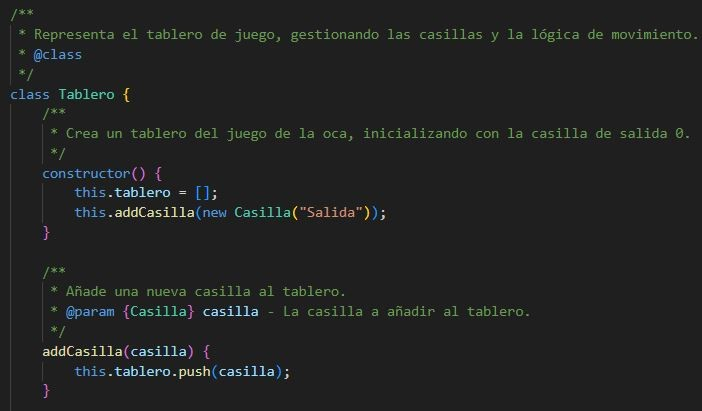
\includegraphics[width=0.82\textwidth]{imgs/codigo-tablero-1.jpg}
	\caption{Declaración de la clase Tablero}
	\label{fig:codigo-tablero-1}
\end{figure}

\newpage
Además, es la encargada de calcular una nueva posición a partir del índice de la casilla actual y el número de desplazamiento, asegurándose de que si es mayor que el número de casillas restantes hasta la meta, pueda retroceder y no salirse del límite.

Otra de sus funcionalidades es la de buscar la siguiente casilla de tipo oca, dada la posición de la actual, útil para manejar el evento cuando se cae en una. También cuenta con un método para obtener la otra casilla de puente.

\begin{figure}[H]
	\centering
	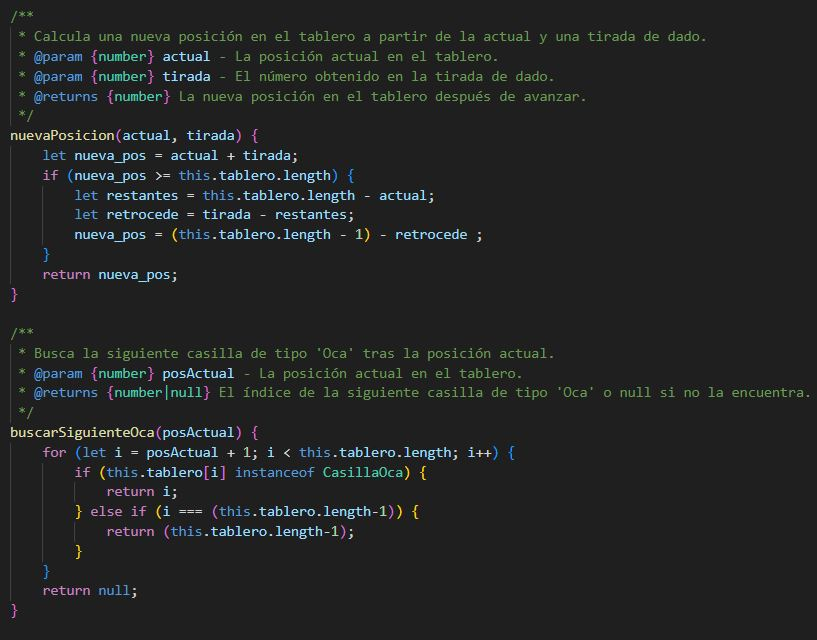
\includegraphics[width=0.9\textwidth]{imgs/codigo-tablero-2.jpg}
	\caption{Métodos para calcular una posición y buscar un tipo de casilla}
	\label{fig:codigo-tablero-2}
\end{figure}

\newpage
\paragraph{Fichero \enquote{EstadoJuego.js}}

Aquí va el contenido del párrafo.

\begin{figure}[H]
	\centering
	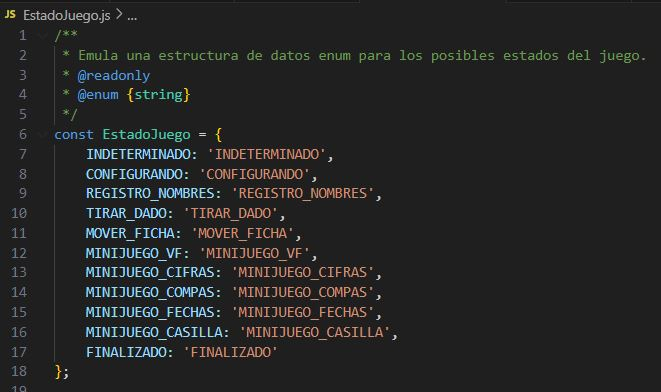
\includegraphics{imgs/codigo-estado-1.jpg}
	\caption{Simula la estructura de datos \textit{enum} de los estados del juego}
	\label{fig:codigo-estado-1}
\end{figure}

\begin{figure}[H]
	\centering
	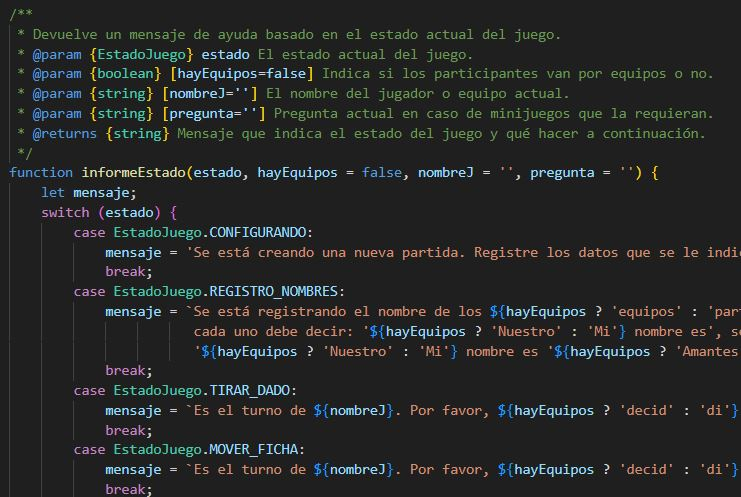
\includegraphics{imgs/codigo-estado-2.jpg}
	\caption{Función que devuelve un mensaje de ayuda según el estado del juego}
	\label{fig:codigo-estado-2}
\end{figure}

\paragraph{Fichero \enquote{JuegoOca.js}}

Es la clase más extensa de todas, haciendo uso del resto de clases definidas anteriormente, lo que puede observarse en los módulos que han tenido que importarse.

\begin{figure}[H]
	\centering
	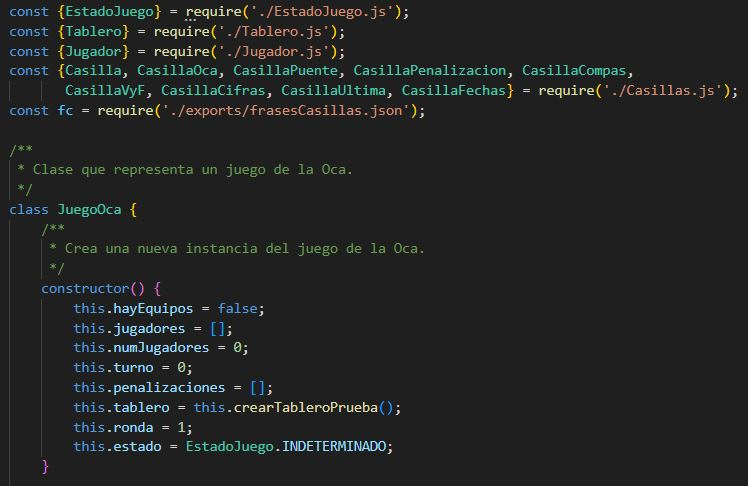
\includegraphics{imgs/codigo-oca-1.jpg}
	\caption{Importaciones y declaración de la clase del juego de la oca}
	\label{fig:codigo-oca-1}
\end{figure}

Esta clase dispone de varios de métodos para implementar la lógica del juego:

\begin{itemize}
	\item \textbf{crearJugadores()}: crea un número específico de jugadores (hasta 5), asignándoles colores y códigos únicos (salvo los nombres, que serán añadidos más tarde), inicializándolos con los valores de partida predeterminados, y actualizando el estado de juego.
	\begin{figure}[H]
		\centering
		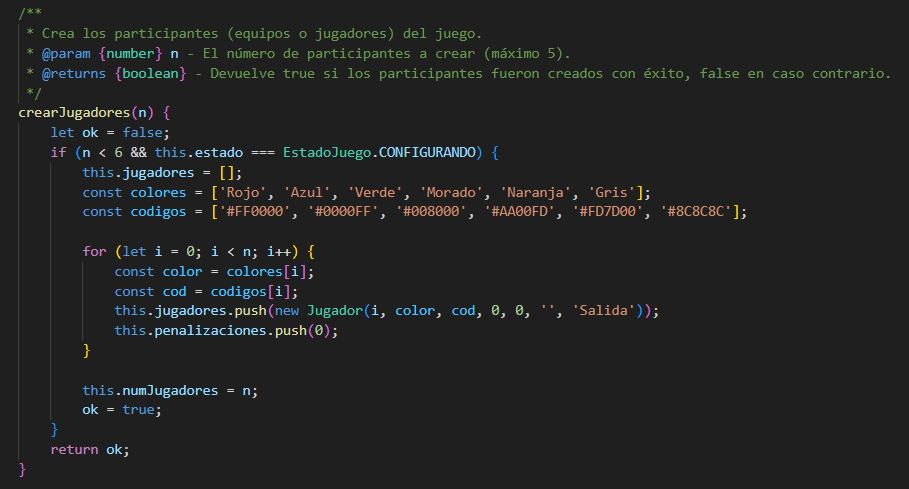
\includegraphics{imgs/codigo-oca-2.jpg}
		\caption{Método de inicialización de participantes del juego}
		\label{fig:codigo-oca-2}
	\end{figure}
	
	\item \textbf{crearTablero()}: genera un tablero completo con 63 casillas, con diferentes tipos como CasillaOca, CasillaPenalizacion, CasillaVyF, entre otras, para un juego completo de la oca.
	\begin{figure}[H]
		\centering
		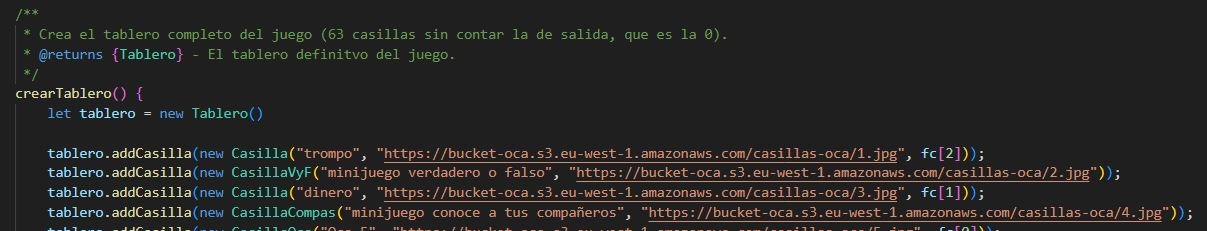
\includegraphics[width=1\textwidth]{imgs/codigo-oca-3.jpg}
		\caption{Método de inicialización del tablero de la oca}
		\label{fig:codigo-oca-3}
	\end{figure}
	
	\item \textbf{pasarTurno()}: avanza el turno, recalcula el número de ronda, actualiza el estado del juego y devuelve un mensaje anunciando el turno del siguiente participante. comprobando antes si tiene penalizaciones de turno o no.
	\begin{figure}[H]
		\centering
		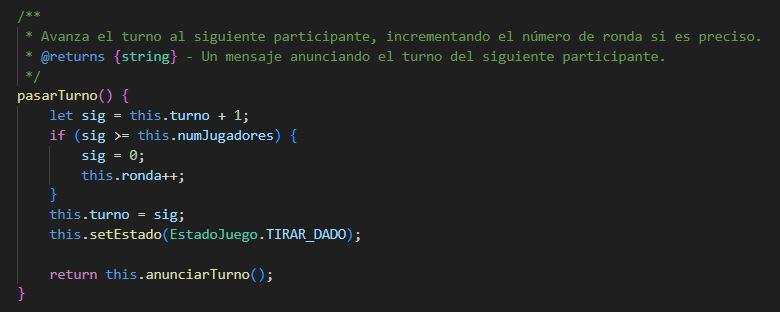
\includegraphics{imgs/codigo-oca-5.jpg}
		\caption{Método para pasar al siguiente turno}
		\label{fig:codigo-oca-5}
	\end{figure} 
	
	\item \textbf{anunciarGanadores()}: si el juego ha finalizado, devuelve u mensaje anunciando las dos modalidades de ganadores: quien haya llegado antes a la meta y quien haya obtenido más puntos gracias a los minijuegos.
	\begin{figure}[H]
		\centering
		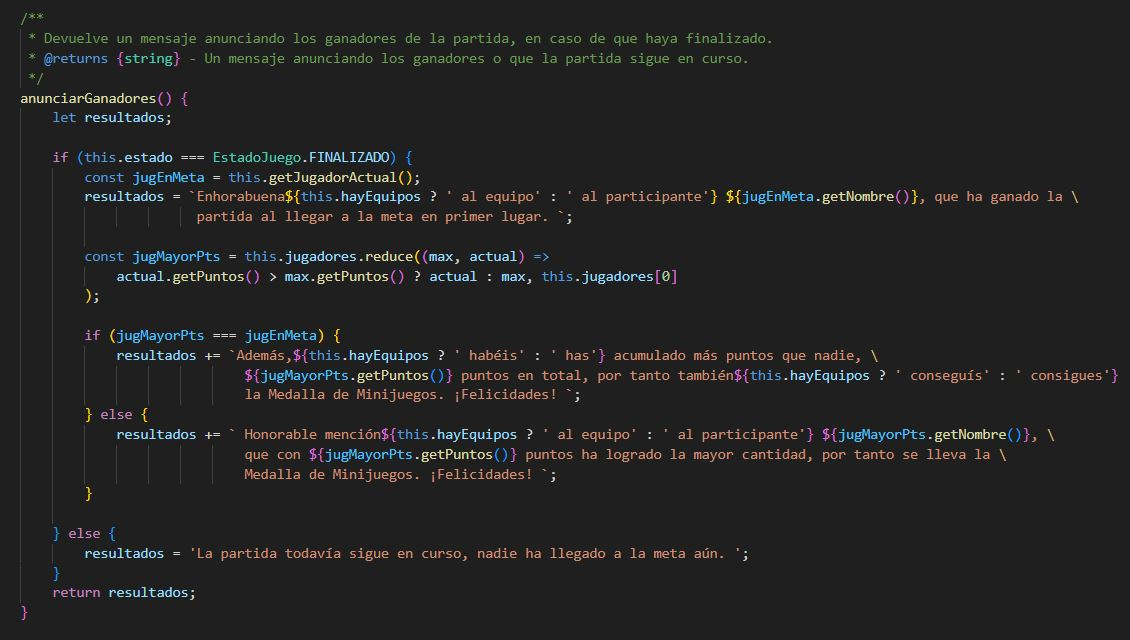
\includegraphics[width=1\textwidth]{imgs/codigo-oca-6.jpg}
		\caption{Método para anunciar los ganadores al final del juego}
		\label{fig:codigo-oca-6}
	\end{figure} 
	 
	\item \textbf{avanzarJugador()}: mueve al participante actual una cantidad determinada de casillas, actualizando su posición y manejando eventos específicos basados en el tipo de casilla en la que cae. También genera un informe sobre el movimiento realizado y actualiza el estado de la partida. \newline
	
	\begin{figure}[H]
		\centering
		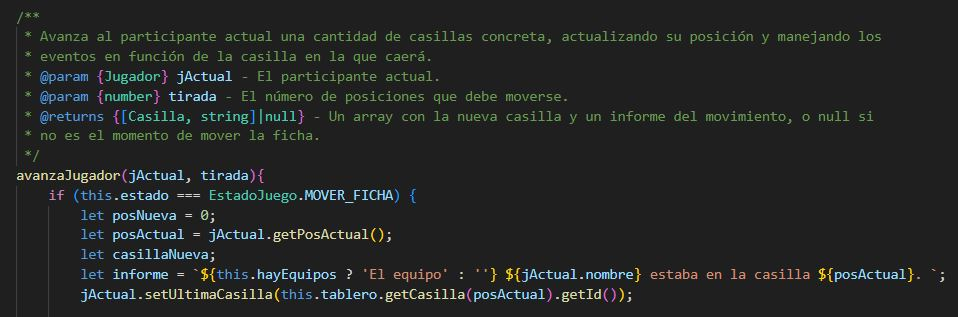
\includegraphics{imgs/codigo-oca-4.jpg}
		\caption{Primeras líneas del método para avanzar las fichas}
		\label{fig:codigo-oca-4}
	\end{figure}
	
	\item Métodos \textit{getters} y \textit{setters} de todos los atributos de la clase.
	\item Métodos adicionales para calcular y hallar: un participante de índice concreto, el equipo o jugador/a del turno actual, sus compañeros de juego, los que se encuentran en una casilla determinada, las penalizaciones de alguno en particular, etc.
\end{itemize}

\subsubsection{Fichero \enquote{handlers.js}}

Con diferencia el fichero más extenso, con unas 900 líneas de código

\begin{figure}[H]
	\centering
	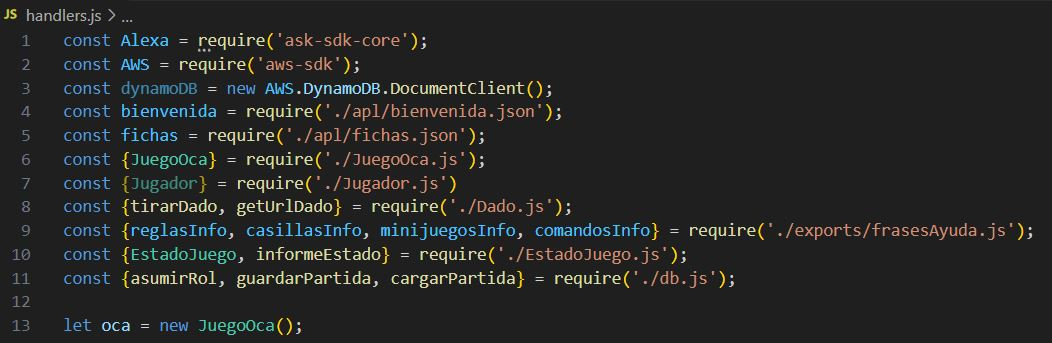
\includegraphics[width=1\textwidth]{imgs/codigo-handlers-1.jpg}
	\caption{Importaciones de bibliotecas y módulos para los handlers}
	\label{fig:codigo-handlers-1}
\end{figure}

De la siguiente lista de handlers definidos, se van a explicar todos los que han sido personalizados de alguna forma, exceptuando aquellos mencionados en la sección \textit{7.1.} que no hayan sufrido ningún cambio.
\begin{figure}[H]
	\centering
	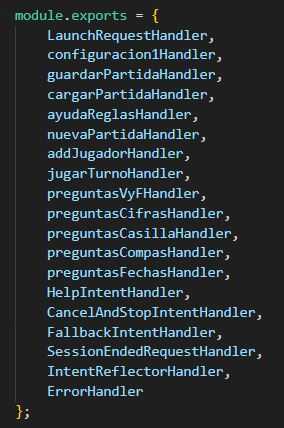
\includegraphics[width=0.4\textwidth]{imgs/codigo-handlers-2.jpg}
	\caption{Todos los handlers que se exportan al \textit{index.js}}
	\label{fig:codigo-handlers-2}
\end{figure}

Cabe mencionar que cada handler está vinculado a un intent con el mismo nombre, que es invocado mediante utterances. Por ejemplo: con la utterance \enquote{Nueva partida}, se activa la intención \textit{nuevaPartidaIntent}, que provocará la ejecución del manejador \textit{nuevaPartidaHandler}, devolviendo una respuesta procesada a la persona usuaria.

\paragraph{\textit{LaunchRequestHandler}}

Este handler se activa cuando el usuario abre la skill por primera vez, mediante el comando \enquote{Alexa, abre probando oca}. Su función principal es dar una bienvenida al usuario y proporcionar opciones iniciales sobre cómo comenzar una partida. Informa al usuario sobre la posibilidad de continuar una partida previamente guardada o iniciar una nueva, advirtiendo que al comenzar una nueva se sobrescribirá la partida anterior. 

Si el dispositivo donde se ejecuta dispone de pantalla, se muestra la pantalla de inicio/bienvenida. Finalmente, el handler prepara una respuesta para que el usuario se sienta guiado sobre los próximos pasos, manteniendo la sesión activa para una interacción más fluida.

\paragraph{\textit{configuracion1Handler}}

Se invoca cuando el usuario solicita un intent específico para configurar una partida de prueba, útil para el proceso de depuración de errores y testeo de la skill. Este handler omite el proceso normal de configuración del juego y establece un estado predeterminado con dos equipos ficticios con nombres y puntos predefinidos para facilitar las pruebas. 

A continuación, notifica al usuario que la partida ha comenzado y le recuerda los comandos necesarios para jugar. Además, muestra información visual sobre los jugadores utilizando directivas APL.

\paragraph{\textit{guardarPartidaHandler} y \textit{cargarPartidaHandler}}

El primero responde a la solicitud de guardar el progreso actual del juego. A través de un rol temporal en AWS, accede a DynamoDB y almacena los datos de la partida en curso. Una vez que la partida se guarda correctamente, confirma el éxito o fracaso de la operación.

El segundo realiza el proceso inverso, pues se activa cuando el usuario desea cargar una partida previamente guardada. Vuelve a asumir un rol IAM temporal para conectarse con DynamoDB y recuperar los datos de la partida guardada. Así, permite continuar jugando desde el última punto guardado. 

\paragraph{\textit{ayudasReglasHandler}}

Invocado cuando la persona usuaria solicita ayuda, mediante el comando \enquote{Explícame <tema>}.

Dependiendo del tema específico sobre el que se quiere recibir información (como reglas generales, casillas del tablero, minijuegos o comandos), el handler proporciona una explicación detallada. Como en el resto de handlers, mantiene la sesión activa para ofrecer asistencia continua y mejorar la experiencia del usuario.

\paragraph{\textit{nuevaPartidaHandler}}

Se encarga de crear una nueva partida cuando el usuario lo solicita. Primero, pregunta por el tipo de participación (individual o en equipos) y luego por el número de participantes desde los slots del intent. 

Una vez se han recibido los datos, y confirmado que son correctos, se actualiza el estado del juego y se proporciona una explicación sobre cómo proceder al registro los nombres, indicando el formato correcto y sugiriendo ejemplos. 

A partir de este punto, se tiene en cuenta el tipo de participación para ajustar todas las respuestas con menciones a los equipos o jugadores individuales. 

\paragraph{\textit{addJugadorHandler}}

Es el paso obligatorio que sigue al anterior handler, este gestiona el registro de nombres de los jugadores en el juego. Se activa cuando cada participante proporciona su nombre a través del comando \enquote{Mi/Nuestro nombre es <nombre>}. 

Primero, verifica si el estado del juego está en la fase de registro de nombres y después, guarda el nombre. Si aún faltan participantes por registrar, solicita el siguiente nombre, y una vez que haya recibido todos, hace un resumen de los jugadores o equipos y guarda los datos de partida configurados en DynamoDB. También muestra en pantalla mediante APL los nombres y colores de los participantes recién registrados.

Por último, informa al usuario que la partida está lista para comenzar y guía sobre los próximos pasos: el lanzamiento de dado y movimiento de ficha.

\paragraph{\textit{jugarTurnoHandler}}

Procesa el turno del participante actual, dividido en dos fases: tirar el dado y mover la ficha. Primero, revisa si el dado ha sido lanzado (el valor del dado de atributo de sesión no es nulo) y en caso contrario, lo lanza y guarda el resultado.

Si el dado ya fue lanzado,realiza el movimiento del jugador en el tablero, avazando su ficha tantas casillas indica el dado y describiendo la casilla en la que ha caído. Dependiendo del tipo que sea, presenta instrucciones específicas sobre cómo proceder.

Por no mencionar que es el encargado de actualizar la interfaz de usuario con información visual sobre la casilla actual y quién está en ella. 
Una vez gestionados los eventos de la nueva casilla, se actualiza el turno actual junto con el estado del juego.

\paragraph{Handlers de minijuegos}

Los cinco handlers que gestionan las preguntadas de cada tipo de minijuego se rigen por un esquema general similar.

\begin{enumerate}
	\item Se comprueba que el estado del juego se corresponde con el del minijuego invocado, para evitar acceder a estos handlers fuera de turno. Si el estado no es el esperado, lanza un mensaje de error y recordatorio de cómo se debe proceder.
	\item Se obtiene la respuesta del participante a través del sistema de slots del intent, que permiten capturar tipos de datos predefinidos.
	\item Se recuperan los datos de la pregunta si es necesario, mediante atributos de sesión, en caso de que Alexa tenga que formularla de nuevo.
	\item Se procede con la verificación de la respuesta.
\end{enumerate}

Es en el paso 4 de la secuencia anterior donde la implementación difiere según el tipo de minijuego del que se trata:

\begin{itemize}
	\item \textbf{preguntasVyFHandler}: compara la respuesta del participante actual (verdadero o falso) con la solución almacenada en forma de booleano. Si coinciden, se suman 10 puntos, si no, ofrece una breve explicación de la respuesta correcta.
	\item \textbf{preguntasCifrasHandler}: compara el número indicado por el participante actual con la solución en formato de entero. Si coinciden, obtiene 30 puntos, y si no, vuelve a formular la pregunta al siguiente. Así hasta que alguien acierte o se haya preguntado a todos y ninguna respuesta haya sido la correcta, en cuyo caso se revela la solución.
	\item \textbf{preguntasCasillaHandler}: compara la respuesta proporcionada, que es un nombre de casilla, con el ID de su última casilla almacenada. Si coinciden, suma 25 puntos, si no, Alexa revela cuál era.
	\item \textbf{preguntasCompasHandler}: primero se guarda la respuesta (formato: correcto/a o incorrecto/a) del participante, y después Alexa le pide al compañero sobre el que iba la pregunta que valide si la respuesta ofrecida era correcta o incorrecta. Si es correcta, ambos ganan 15 puntos.
	\item \textbf{preguntasFechasHandler}: compara la respuesta del participante actual (día, mes o estación), con la fecha calculada correcta. Si coincide, se suman 20 puntos.
\end{itemize}

\paragraph{\textit{ErrorHandler}}

Se ha incluido una comprobación del estado actual del juego, para que pueda adaptar correctamente el mensaje de error a cada situación.

Si el estado indica que uno de los minijuegos está en curso, el mensaje de error incluirá información específica sobre la pregunta actual, y si no, serán instrucciones más fijas en base a dicho estado. Por ejemplo, si es el inicio del turno de algún participante, pero Alexa no recibe respuesta en un tiempo determinado o se intenta acceder a un comando no permitido, Alexa le recordará que es tiene que tirar el dado y cómo debe hacerlo.

\subsubsection{Fichero \enquote{index.js}}

Explicado previamente en la sección 7.1., se ha modificado para incluir todas las funciones manejadoras definidas hasta ahora.

\begin{figure}[H]
	\centering
	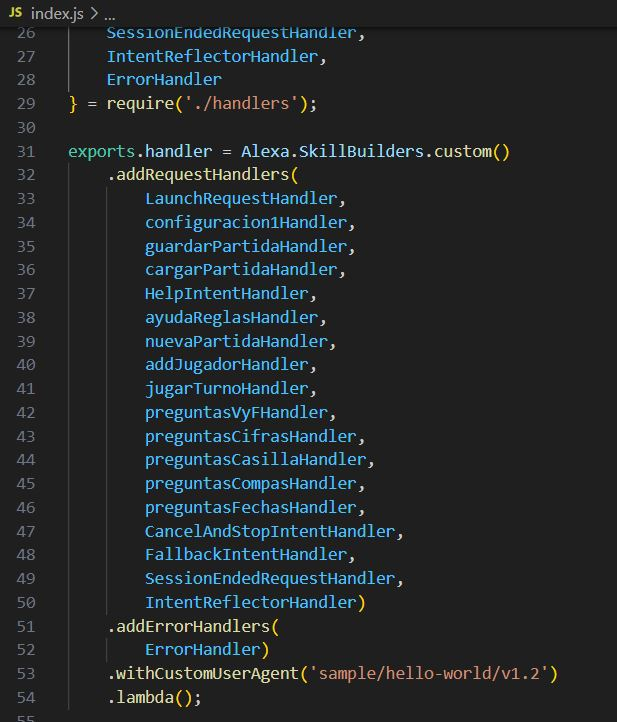
\includegraphics{imgs/codigo-index.jpg}
	\caption{Exportación de manejadores a la función Lambda}
	\label{fig:codigo-index}
\end{figure}

\subsubsection{Directorio \enquote{apl}}

Se tiene la siguiente estructura de ficheros JSON para la configuración de directivas de APL dentro de la respuesta de los manejadores:
\begin{figure}[H]
	\centering
	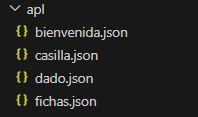
\includegraphics[width=0.4\textwidth]{imgs/apl-carpeta.jpg}
	\caption{Directorio de ficheros JSON para APL}
	\label{fig:apl-carpeta}
\end{figure}

\paragraph{\textit{bienvenida.json}}

Es la pantalla de inicio, es decir, el aspecto que toma nada más iniciar la skill, compuesto por una imagen y un texto de bienvenida.

\begin{figure}[H]
	\centering
	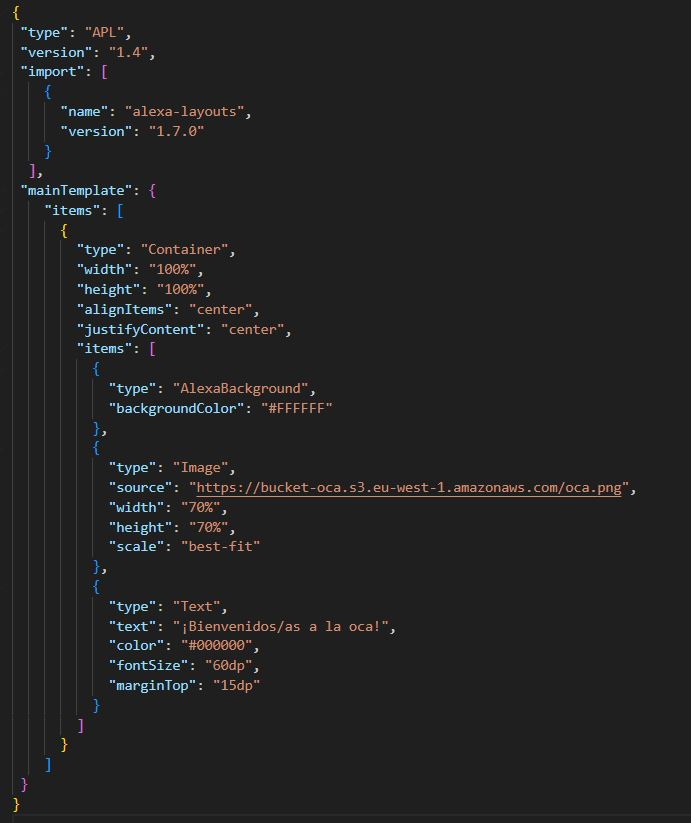
\includegraphics[width=0.9\textwidth]{imgs/apl-bienvenida.jpg}
	\caption{Documento APL para la pantalla de inicio}
	\label{fig:apl-bienvenida}
\end{figure}

\begin{figure}[H]
	\centering
	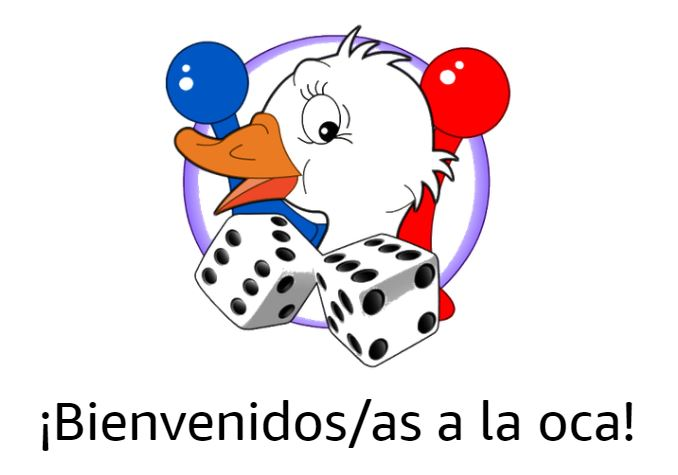
\includegraphics{imgs/interfaz-1.jpg}
	\caption{Pantalla de bienvenida de la skill}
	\label{fig:interfaz-1}
\end{figure}

\paragraph{\textit{fichas.json}}

Aparece tras configurar la partida que se va a jugar, con los participante ya registrados. Simplemente muestra los nombres de cada equipo o jugador/a, junto con el color que tienen asociado.

\begin{figure}[H]
	\centering
	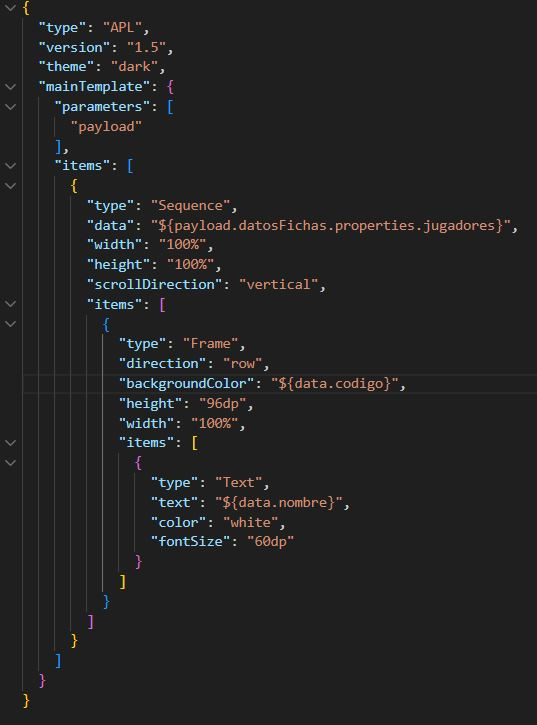
\includegraphics[width=0.8\textwidth]{imgs/apl-fichas.jpg}
	\caption{Documento APL para mostrar los participantes del juego}
	\label{fig:apl-fichas}
\end{figure}

\begin{figure}[H]
	\centering
	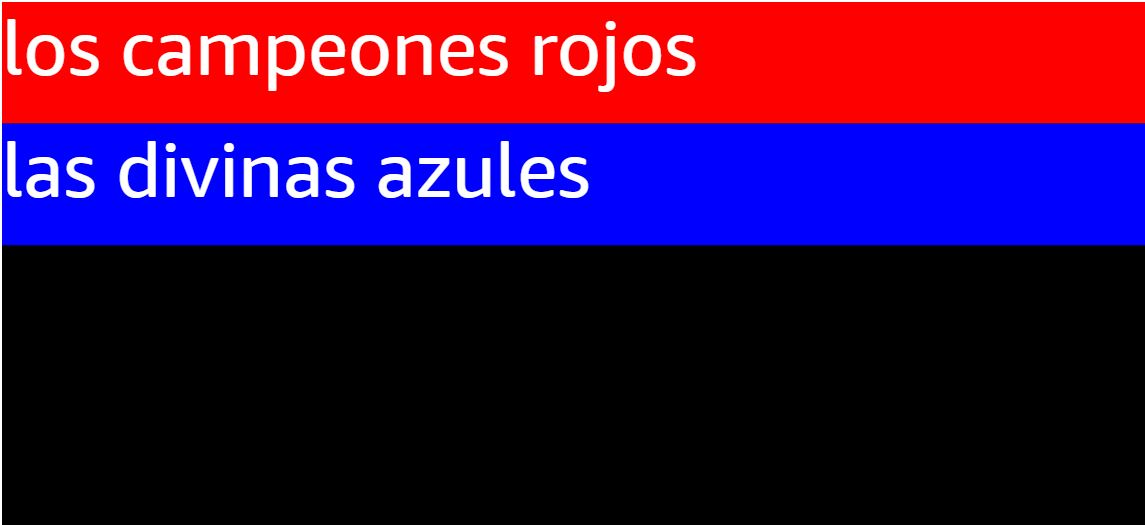
\includegraphics[width=0.8\textwidth]{imgs/interfaz-2.jpg}
	\caption{Pantalla postconfiguración mostrando a los participante}
	\label{fig:interfaz-2}
\end{figure}

\paragraph{\textit{dado.json}}

Utilizado después de cada lanzamiento de dado para reproducir la animación correspondiente al número obtenido en la tirada (hay seis vídeos en total, uno para cada resultado).

\begin{figure}[H]
	\centering
	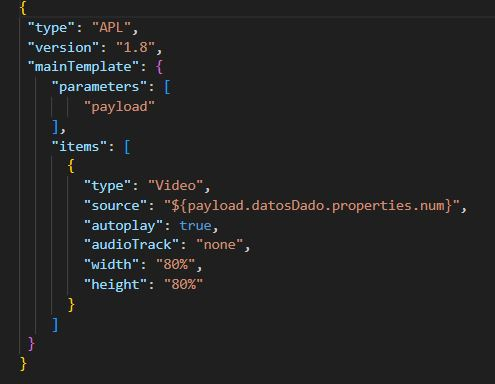
\includegraphics[width=0.7\textwidth]{imgs/apl-dado.jpg}
	\caption{Documento APL para mostrar la animación del dado}
	\label{fig:apl-dado}
\end{figure}

\begin{figure}[H]
	\centering
	
\includegraphics{imgs/interfaz-3.jpg}
	\caption{Pantalla mostrando un lanzamiento de dado}
	\label{fig:interfaz-3}
\end{figure}

\paragraph{\textit{casilla.json}}

Muestra en la mitad izquierda los participantes que están en esa casilla, pudiendo haber más de uno en la misma, y en la mitad derecha, la imagen asociada a la casilla con su número o índice dentro del tablero.

\begin{figure}[H]
	\centering
	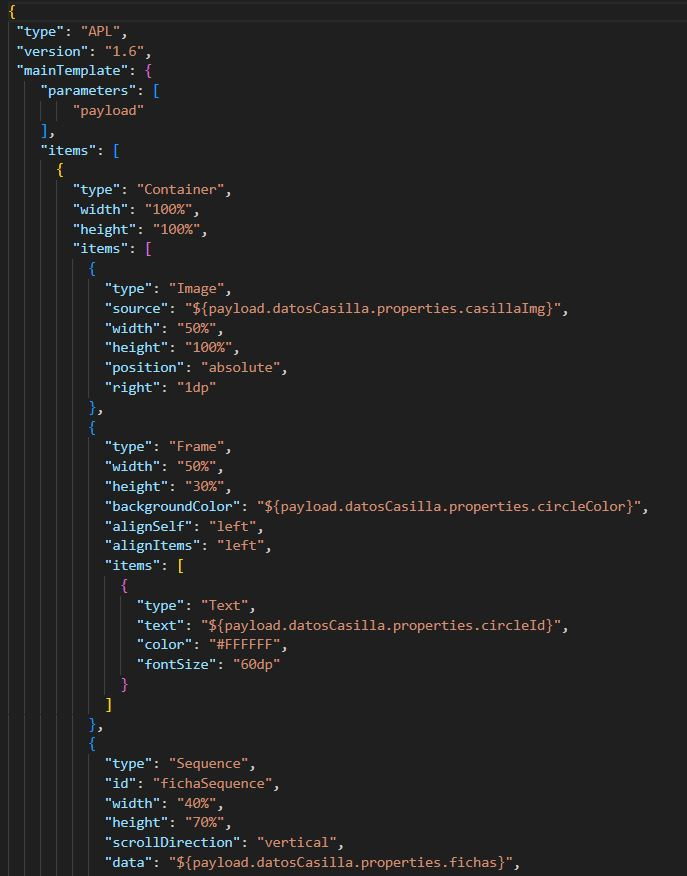
\includegraphics[width=0.85\textwidth]{imgs/apl-casilla.jpg}
	\caption{Documento APL para mostrar la casilla y participante actuales}
	\label{fig:apl-casilla}
\end{figure}

\begin{figure}[H]
	\centering
	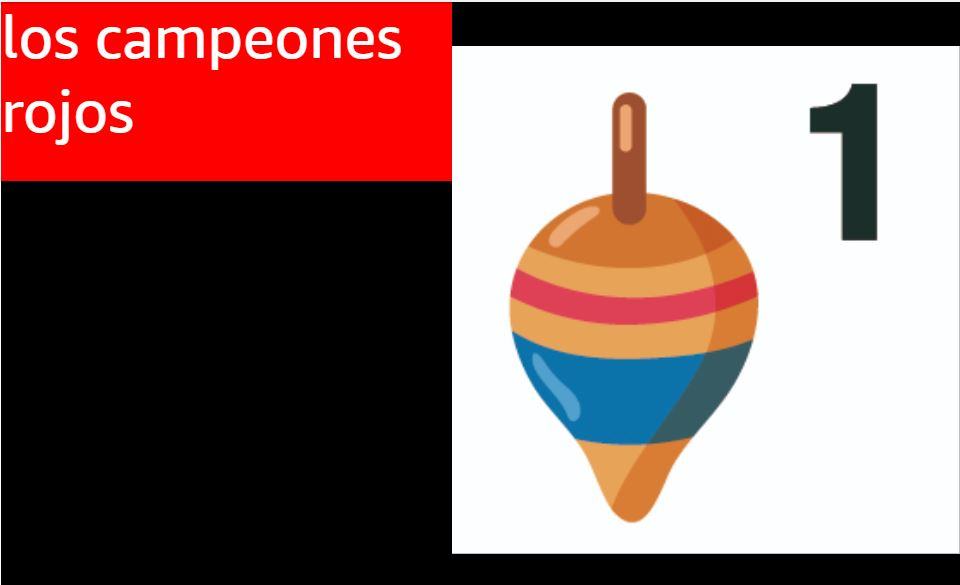
\includegraphics[width=0.8\textwidth]{imgs/interfaz-4.jpg}
	\caption{Pantalla mostrando la casilla y participante actuales}
	\label{fig:interfaz-4}
\end{figure}

\subsubsection{Directorio \enquote{exports}}

En esta carpeta se encuentran aquellos datos que van a ser importados en otros módulos, como por ejemplo las baterías de preguntas de los minijuegos o las frases aleatorias de las casillas normales.

\begin{figure}[H]
	\centering
	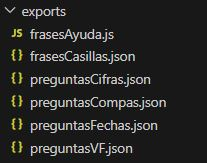
\includegraphics[width=0.4\textwidth]{imgs/exp-carpeta.jpg}
	\caption{Directorio de ficheros exportados a otros módulos}
	\label{fig:exp-carpeta}
\end{figure}

\paragraph{\textit{frasesAyuda.js}}

Contiene las descripciones de los distintos temas de los que puede solicitarse una explicación a través de \textit{ayudaReglasIntent}. Hay una variable constante en formato cadena de texto para cada tema posible: las reglas del juego, los tipos de casilla, los minijuegos y los comandos disponibles.

\paragraph{\textit{frasesCasillas.json}}

Es donde viene almacenada la información de las casillas de tipo normal. Los datos relevantes son: el identificador (id) o nombre de la casilla, el número o índice dentro del tablero y un arreglo de frases posibles para recibir a cada modalidad de participante (individual o equipo).

\begin{figure}[H]
	\centering
	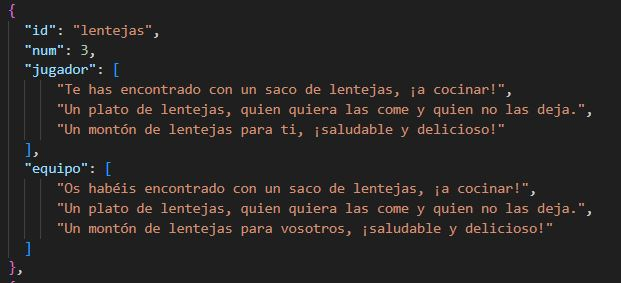
\includegraphics[width=0.7\textwidth]{imgs/exp-casillas.jpg}
	\caption{Ejemplo de objeto con la información de una casilla normal}
	\label{fig:exp-casillas}
\end{figure}

\paragraph{\textit{preguntasCifras.json}}

El conjunto de preguntas posibles para el minijuego de adivinar la cifra, compuestas por el texto de la pregunta en sí y su solución, que siempre es un número entero.

\begin{figure}[H]
	\centering
	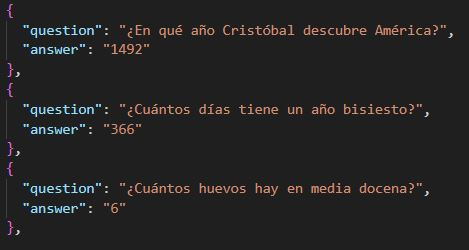
\includegraphics[width=0.7\textwidth]{imgs/exp-cifras.jpg}
	\caption{Ejemplos de preguntas en \enquote{Adivina la cifra}}
	\label{fig:exp-cifras}
\end{figure}

\newpage
\paragraph{\textit{preguntasVF.json}}

La batería de preguntas de tipo trivial verdadero o falso, compuestas por el texto de la pregunta en, su solución (booleano) y una explicación de la respuesta que se mencionará si se falla.

\begin{figure}[H]
	\centering
	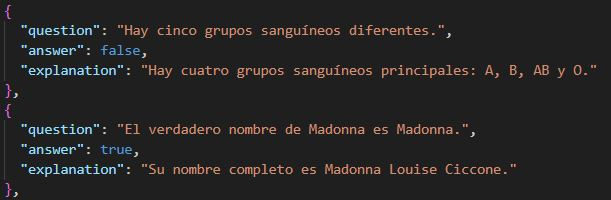
\includegraphics[width=0.7\textwidth]{imgs/exp-vyf.jpg}
	\caption{Ejemplos de preguntas de \enquote{Verdadero o falso}}
	\label{fig:exp-vyf}
\end{figure}

\paragraph{\textit{preguntasCompas.json}}

Todas las preguntas acerca del resto de participantes que pueden salir en el minijuego de conoce a tus compañeros. Cada objeto se compone de un texto de la pregunta para cada tipo de participante (equipos o individuales).

\begin{figure}[H]
	\centering
	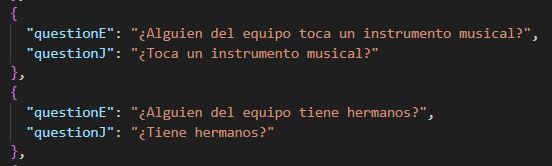
\includegraphics[width=0.7\textwidth]{imgs/exp-compas.jpg}
	\caption{Ejemplos de preguntas acerca de los compañeros de juego}
	\label{fig:exp-compas}
\end{figure}

\paragraph{\textit{preguntasFechas.json}}

El conjunto de posibles preguntas de fechas, cada objeto definido por tres atributos: el tipo de pregunta, que indica a su vez el tipo de respuesta esperada (día de la semana, mes o estación del año), el texto de la pregunta y el id o número de desplazamiento que hay que aplicar sobre la fecha actual para calcular la respuesta correcta.

\begin{figure}[H]
	\centering
	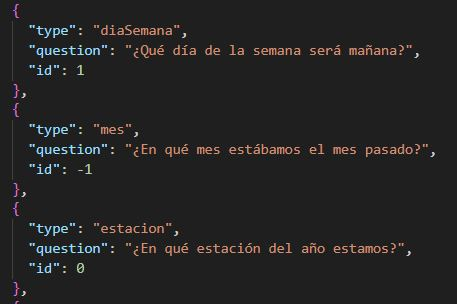
\includegraphics[width=0.7\textwidth]{imgs/exp-fechas.jpg}
	\caption{Ejemplos de preguntas acerca en \enquote{Recuerda la fecha}}
	\label{fig:exp-fechas}
\end{figure}

En los tres ejemplos anteriores, las soluciones son dinámicas y se calcularían empleando los métodos de la clase \textit{CasillaFechas} encargados de aplicar el desplazamiento indicado por el id sobre el valor de la fecha actual (una instancia nueva de \textit{Date}). Por ejemplo, si se hace la pregunta el primer jueves de enero en España, la respuesta a cada una sería: viernes, diciembre e invierno.

\subsubsection{Fichero \enquote{db.js}}

Como indica el nombre del fichero, incluirá todas las funciones relativas a operaciones con elementos de las tablas alojadas en DynamoDB. Se destacan las tres principales:

\paragraph{\textit{asumirRol()}}

Permite asumir un rol de AWS para obtener credenciales temporales para poder acceder a DynamoDB de forma segura. Se han seguido los pasos de una de las guías de la documentación oficial de Alexa \parencite{alexaHosted2}:

\begin{enumerate}
	\item Crear una instancia de cliente STS (\textit{Security Token Service}) usando \textit{AWS.STS}.
	\item Se llama al método \textit{assumeRole()} del cliente STS, proporcionando el ARN del rol que se desea asumir y un nombre para la sesión. Este devuelve credenciales temporales (\textit{AccessKeyId}, \textit{SecretAccessKey} y \textit{SessionToken}).
	\item Se termina de configurar el nuevo cliente \textit{DynamoDB.DocumentClient}, utilizando las credenciales temporales obtenidas en el paso previo, que será el objeto que devuelve la función.
\end{enumerate}

\begin{figure}[H]
	\centering
	\includegraphics{imgs/codigo-db-1.jpg}
	\caption{Función para asumir un rol IAM con permisos temporales}
	\label{fig:codigo-db-1}
\end{figure}

\paragraph{\textit{guardarPartida()}}

Almacena los detalles de una partida en la tabla \textit{JuegoOca} y la información de los jugadores en la tabla \textit{Jugador} en DynamoDB, de la siguiente forma:
\begin{enumerate}
	\item Prepara un objeto \textit{params} para guardar los datos generales de la partida en la tabla \textit{JuegoOca}: estado, número de jugadores, ronda y turno. 
	\item Se usa el método \textit{put} del cliente DynamoDB para guardar la información de la partida en la tabla, permitiendo capturar cualquier error que surja durante este proceso.
	\item Llama a la función \textit{guardarJugadores()}, encargada de repetir el mismo proceso seguido en los dos pasos anteriores, pero esta vez con los datos de cada participante: nombre, color, puntos, posición, etc.
	\item Los resultados de ambas operaciones de guardado se concatenan en un mensaje de texto puramente informativo que será el devuelto por la función.
\end{enumerate}

\begin{figure}[H]
	\centering
	\includegraphics{imgs/codigo-db-2.jpg}
	\caption{Función para guardar los datos de la partida en DynamoDB}
	\label{fig:codigo-db-2}
\end{figure}

\paragraph{\textit{cargarPartida()}}

Leva a cabo el proceso anterior pero en sentido contrario, dicho en otras palabras, recupera la información desde la tabla de DynamoDB y la carga en en contexto de la skill de Alexa.
\begin{enumerate}
	\item Se configura un objeto \textit{params} para obtener los datos generales de la partida con la clave primaria, \textit{idJuego}, de la tabla \textit{JuegoOca}. 
	\item Se usa el método \textit{get} del cliente DynamoDB para cargar la información de la partida, y si esta es válida, se actualizan los datos de la instancia actual de \textit{JuegoOca}.
	\item Invoca la función \textit{cargarJugadores()}, para repetir el proceso de los pasos 1 y 2, esta vez usando la clave primaria \textit{idJugador}, que coincide con el ID de cada participante.
	\item La función devuelve los informes de éxito o fracaso de ambas operaciones de carga de datos.
\end{enumerate}

\begin{figure}[H]
	\centering
	\includegraphics{imgs/codigo-db-3.jpg}
	\caption{Función para cargar los datos de la partida desde DynamoDB}
	\label{fig:codigo-db-3}
\end{figure}

\newpage

\subsection{Pruebas}

Para verificar la correcta implementación de la skill, es vital probar cada uno de los módulos por separado (pruebas unitarias), y después en conjunto (pruebas de integración). Dichas pruebas se enumeran en las siguientes secciones.

\subsubsection{Pruebas unitarias}

Las pruebas unitarias permiten verificar que cada componente, en este caso, cada función manejadora o handler de la skill, funciona correctamente al ejecutarse de forma aislada.

\begin{table}[H]
	\centering
	\begin{tabular}{|c|p{8.5cm}|}
		\hline
		\rowcolor{lightgray}
		\multicolumn{2}{|c|}{\textbf{PU01}: Lanzar skill y pantalla de inicio} \\
		\hline
		\textbf{Descripción} & Se dice: <<Alexa, abre probando oca>> \vspace{0.2cm} \\
		\hline
		\textbf{Resultado esperado} & Se inicia la skill, mostrando la pantalla de inicio y un mensaje de bienvenida. \vspace{0.2cm} \\
		\hline
		\textbf{Resultado obtenido} & Alexa da un mensaje de bienvenida, indicaciones básicas para empezar a jugar y se muestra por pantalla el logo del juego con un texto de bienvenida. \vspace{0.2cm} \\
		\hline
		\textbf{CU referenciado(s)} & CU01 \vspace{0.2cm} \\
		\hline
		\textbf{Estado de validación} & Aprobado \vspace{0.2cm} \\
		\hline
	\end{tabular}
	\caption{Prueba unitaria nº 1}
	\label{tab:PU01}
\end{table}


\begin{table}[H]
	\centering
	\begin{tabular}{|c|p{8.5cm}|}
		\hline
		\rowcolor{lightgray}
		\multicolumn{2}{|c|}{\textbf{PU02}: Probar los comandos de ayuda} \\
		\hline
		\textbf{Descripción} & Se dice <<Ayuda>>, y después <<Explícame las reglas>> \vspace{0.2cm} \\
		\hline
		\textbf{Resultado esperado} & Un listado de los temas de ayuda disponibles, y la explicación de las reglas. \vspace{0.2cm} \\
		\hline
		\textbf{Resultado obtenido} & Primero Alexa lista los temas que puede elaborar. Luego procede a explicar el tema que se ha pedido (las reglas del juego), detallando los objetivos principales del juego. \vspace{0.2cm} \\
		\hline
		\textbf{CU referenciado(s)} & CU02 \vspace{0.2cm} \\
		\hline
		\textbf{Estado de validación} & Aprobado \vspace{0.2cm} \\
		\hline
	\end{tabular}
	\caption{Prueba unitaria nº 2}
	\label{tab:PU02}
\end{table}

\begin{table}[H]
	\centering
	\begin{tabular}{|c|p{8.5cm}|}
		\hline
		\rowcolor{lightgray}
		\multicolumn{2}{|c|}{\textbf{PU03}: Crear una partida nueva} \\
		\hline
		\textbf{Descripción} & Se dice: <<Nueva partida>> \vspace{0.2cm} \\
		\hline
		\textbf{Resultado esperado} & Alexa va preguntando los datos necesarios para configurar la partida. Cuando tenga todos, muestra a los y las participantes, y marca el inicio del juego.  \vspace{0.2cm} \\
		\hline
		\textbf{Resultado obtenido} & Alexa pregunta por los datos de la partida, en el siguiente orden: tipo de participante, número de ellos y el nombre de cada uno. Tras lo cual hace un resumen de los participantes, mostrando por pantalla la información de cada uno, y anuncia el primer turno. \vspace{0.2cm} \\
		\hline
		\textbf{CU referenciado(s)} & CU03 y CU04 \vspace{0.2cm} \\
		\hline
		\textbf{Estado de validación} & Aprobado \vspace{0.2cm} \\
		\hline
	\end{tabular}
	\caption{Prueba unitaria nº 3}
	\label{tab:PU03}
\end{table}

\begin{table}[H]
	\centering
	\begin{tabular}{|c|p{8.5cm}|}
		\hline
		\rowcolor{lightgray}
		\multicolumn{2}{|c|}{\textbf{PU04}: Guardar y cargar la partida} \\
		\hline
		\textbf{Descripción} & 
		\textbf{1.} Con la partida ya configurada, pero antes de tirar el dado, se dice <<Guardar partida>>. \newline
		\vspace{0.2cm}
		\textbf{2.} Se cierra la skill diciendo: <<Cierra probando oca>>. \newline
		\vspace{0.2cm}
		\textbf{3.} Se vuelve a abrir la skill, y se dice: <<Continuar partida>>. \newline
		\vspace{0.2cm} \\
		\hline
		\textbf{Resultado esperado} & Se puede retomar la partida con los datos guardados antes de cerrar la skill.  \vspace{0.2cm} \\
		\hline
		\textbf{Resultado obtenido} & Alexa da un mensaje de éxito, y tras volver a iniciarse la skill y escuchar el comando de carga de datos, confirma el éxito de la operación. Después, recuerda por qué turno se quedó la partida y a quién le toca continuar. \vspace{0.2cm} \\
		\hline
		\textbf{CU referenciado(s)} & CU01, CU06, CU07 y CU13 \vspace{0.2cm} \\
		\hline
		\textbf{Estado de validación} & Aprobado \vspace{0.2cm} \\
		\hline
	\end{tabular}
	\caption{Prueba unitaria nº 4}
	\label{tab:PU04}
\end{table}

Las pruebas realizadas a partir de este punto dan por hecho que se ha iniciado previamente la skill y se ha invocado a \textit{configurarPruebaIntent}, que está asociado a \textit{configuracion1Handler}, que lo que hace es crear una partida con los datos de configuración ya inicializados (un supuesto en el que existen 2 equipos, llamados rojo y azul). 
De esta forma, se evitar tener que repetir la prueba PU03 (ya completada), ahorrando así tiempo para testear el resto de funcionalidades.

\begin{table}[H]
	\centering
	\begin{tabular}{|c|p{8.5cm}|}
		\hline
		\rowcolor{lightgray}
		\multicolumn{2}{|c|}{\textbf{PU05}: Jugar un turno} \\
		\hline
		\textbf{Descripción} & Llegado su turno, el equipo rojo dice <<Tirar dado>>, después, dice <<Mover ficha>>. \vspace{0.2cm} \\
		\hline
		\textbf{Respuesta esperada} & Primero se muestra el lanzamiento del dado y después, la casilla en la que ha caído junto con la información del equipo. A continuación, se dan indicaciones de cómo proceder. \vspace{0.2cm} \\
		\hline
		\textbf{Respuesta obtenida} & Alexa anuncia el resultado de la tirada de dado (un 1) a la vez que muestra dicha animación. Acto seguido, informa sobre el movimiento del equipo rojo desde la casilla actual (salida) a la nueva (casilla normal del trompo en la posición 1 del tablero). 
		
		Se muestra por pantalla la imagen de la casilla del trompo al lado de la ficha del equipo (con su color y nombre) y Alexa dice una de las frases aleatorias para recibir al equipo en esa determinada casilla. \\
		\hline
		\textbf{CU referenciado(s)} & CU05 \vspace{0.2cm} \\
		\hline
		\textbf{Estado de validación} & Aprobado \vspace{0.2cm} \\
		\hline
	\end{tabular}
	\caption{Prueba unitaria nº 5}
	\label{tab:PU05}
\end{table}

Para probar cada minijuego, se ha creado un tablero de prueba reducido con 5 casillas, una de cada minijuego, y se ha forzado el resultado del lanzamiento de dado al valor necesario para caer en cada una de ellas, obligando así a desencadenar el evento a validar.

\begin{table}[H]
	\centering
	\begin{tabular}{|c|p{9.3cm}|}
		\hline
		\rowcolor{lightgray}
		\multicolumn{2}{|c|}{\textbf{PU06}: Minijuego verdadero o falso} \\
		\hline
		\textbf{Descripción} & El equipo rojo cae en la casilla de dicho minijuego y Alexa le hace una pregunta de verdadero o falso que debe responder.
		 \vspace{0.2cm} \\
		\hline
		\textbf{Respuesta esperada} & Alexa verifica si la respuesta del equipo es correcta y actualiza los puntos en caso afirmativo. \vspace{0.2cm} \\
		\hline
		\textbf{Respuesta obtenida} & Si el equipo acierta la pregunta, Alexa da la enhorabuena y suma 10 puntos a su marcador.
		
		Si el equipo la falla, Alexa da una breve explicación de la solución.
		
		En caso de que no reciba respuesta o esta sea de formato incorrecto, Alexa repite la pregunta y el tipo de respuesta válido. \\
		\hline
		\textbf{CU referenciado(s)} & CU08 \vspace{0.2cm} \\
		\hline
		\textbf{Estado de validación} & Aprobado \vspace{0.2cm} \\
		\hline
	\end{tabular}
	\caption{Prueba unitaria nº 6}
	\label{tab:PU06}
\end{table}

\begin{table}[H]
	\centering
	\begin{tabular}{|c|p{9.3cm}|}
		\hline
		\rowcolor{lightgray}
		\multicolumn{2}{|c|}{\textbf{PU07}: Minijuego conoce a tus compañeros} \\
		\hline
		\textbf{Descripción} & El equipo rojo cae en la casilla de dicho minijuego y Alexa le hace una pregunta acerca del equipo azul, que debe responder con <<correcto>> o <<incorrecto>>. Será el propio equipo azul quien valide la respuesta.
		\vspace{0.2cm} \\
		\hline
		\textbf{Respuesta esperada} & Alexa guarda la respuesta del equipo rojo y después le pregunta al equipo azul si es correcto lo que han dicho, actualizando los puntos de ambos en caso afirmativo. \vspace{0.2cm} \\
		\hline
		\textbf{Respuesta obtenida} & Si el equipo azul confirma que la respuesta del equipo rojo es correcta, Alexa da la enhorabuena y suma puntos a ambos.
		
		Si el equipo azul dice que es incorrecto, Alexa da un mensaje de ánimo antes de pasar al siguiente turno.
		
		En caso de que no reciba respuesta o esta sea de formato incorrecto, Alexa repite la pregunta y el tipo de respuesta válido. \\
		\hline
		\textbf{CU referenciado(s)} & CU09 \vspace{0.2cm} \\
		\hline
		\textbf{Estado de validación} & Aprobado \vspace{0.2cm} \\
		\hline
	\end{tabular}
	\caption{Prueba unitaria nº 7}
	\label{tab:PU07}
\end{table}

\begin{table}[H]
	\centering
	\begin{tabular}{|c|p{9.3cm}|}
		\hline
		\rowcolor{lightgray}
		\multicolumn{2}{|c|}{\textbf{PU08}: Minijuego adivina la cifra} \\
		\hline
		\textbf{Descripción} & El equipo rojo cae en la casilla de dicho minijuego y Alexa le hace una pregunta cuya solución es un cifra.
		\vspace{0.2cm} \\
		\hline
		\textbf{Respuesta esperada} & Alexa comprueba si la respuesta del equipo es correcta, dándole puntos en caso afirmativo, y si no lo es, pasa a preguntarle al siguiente equipo. \vspace{0.2cm} \\
		\hline
		\textbf{Respuesta obtenida} & Si el equipo azul acierta la cifra, Alexa da la enhorabuena y le suma 30 puntos.
		
		Si ha fallado, Alexa redirige la pregunta al equipo azul. Si aciertan, se llevan los puntos y si no, Alexa concluye que nadie sabía la solución así que la revela para todos.
		
		En caso de que no reciba respuesta o esta sea de formato incorrecto, Alexa repite la pregunta y el tipo de respuesta válido. \\
		\hline
		\textbf{CU referenciado(s)} & CU10 \vspace{0.2cm} \\
		\hline
		\textbf{Estado de validación} & Aprobado \vspace{0.2cm} \\
		\hline
	\end{tabular}
	\caption{Prueba unitaria nº 8}
	\label{tab:PU08}
\end{table}

\begin{table}[H]
	\centering
	\begin{tabular}{|c|p{9.3cm}|}
		\hline
		\rowcolor{lightgray}
		\multicolumn{2}{|c|}{\textbf{PU09}: Minijuego recuerda la última casilla} \\
		\hline
		\textbf{Descripción} & El equipo rojo, que estaba en la casilla de salida, ahora cae en la casilla de dicho minijuego y Alexa le pregunta cuál fue la última casilla en la que estuvo.
		\vspace{0.2cm} \\
		\hline
		\textbf{Respuesta esperada} & Alexa comprueba si la respuesta del equipo es correcta, dándole puntos en caso afirmativo. \vspace{0.2cm} \\
		\hline
		\textbf{Respuesta obtenida} & Si el equipo azul responde con <<la casilla de salida>>, habrá acertado, por tanto ganará 25 puntos.
		
		Si no sabe la respuesta o se equivoca de casilla, Alexa revelará la solución.
		
		En caso de que la respuesta sea de formato incorrecto, Alexa repite la pregunta y el tipo de respuesta válido. \\
		\hline
		\textbf{CU referenciado(s)} & CU11 \vspace{0.2cm} \\
		\hline
		\textbf{Estado de validación} & Aprobado \vspace{0.2cm} \\
		\hline
	\end{tabular}
	\caption{Prueba unitaria nº 9}
	\label{tab:PU09}
\end{table}

\begin{table}[H]
	\centering
	\begin{tabular}{|c|p{9cm}|}
		\hline
		\rowcolor{lightgray}
		\multicolumn{2}{|c|}{\textbf{PU10}: Minijuego recuerda la fecha} \\
		\hline
		\textbf{Descripción} & El equipo rojo cae en la casilla de dicho minijuego y Alexa le pregunta por un día de la semana, mes o estación que puede ser la actual o calcularse a partir de ella.
		\vspace{0.2cm} \\
		\hline
		\textbf{Respuesta esperada} & Alexa comprueba si la respuesta del equipo es correcta, dándole puntos en caso afirmativo. \vspace{0.2cm} \\
		\hline
		\textbf{Respuesta obtenida} & Si el equipo azul responde con el día de la semana, mes o estación correcta, significará que se ha acordado bien de la fecha actual, y por tanto ganará 20 puntos.
		
		Si falla la pregunta, Alexa revelará la respuesta correcta.
		
		En caso de que la respuesta sea de formato incorrecto, Alexa repite la pregunta y el tipo de respuesta válido. \\
		\hline
		\textbf{CU referenciado(s)} & CU12 \vspace{0.2cm} \\
		\hline
		\textbf{Estado de validación} & Aprobado \vspace{0.2cm} \\
		\hline
	\end{tabular}
	\caption{Prueba unitaria nº 10}
	\label{tab:PU10}
\end{table}

\subsubsection{Pruebas de integración}

Las pruebas de integración sirven para validar el funcionamiento en conjunto de los distintos componentes de la skill. Para ello, una vez probados todos los módulos por separado, se han realizado simulaciones de partidas desde cero. Los pasos seguidos han sido:
\begin{enumerate}
	\item Abrir la skill del juego de la oca.
	\item Decir que cree una nueva partida.
	\item Ir proporcionando los parámetros de configuración: el tipo de participante (por equipos), el número total de ellos (2) y sus nombres (<<los campeones rojos>> y <<las divinas azules>>).
	\item El equipo rojo dice <<tirar dado>>.
	\item Tras obtener un resultado del 1 al 6, dice <<mover ficha>>.
	\item El equipo rojo cae en una casilla normal. Pasa el turno al equipo azul.
	\item El equipo azul tira el dado y mueve su ficha de la misma forma que lo hizo el rojo.
	\item Se gestiona el evento de la casilla en la que ha caído, y pasan a la ronda 2, empezado otra vez por el turno del equipo rojo.
	\item Siguen avanzando por el tablero hasta que uno de ellos llega a la casilla de meta, o si se quiere pausar la partida, se guarda el progreso actual para después retomarlo.
\end{enumerate}

Una forma eficiente de probar la skill en su totalidad es usando el propio simular de Alexa de la consola de desarrollo, tal y como se muestra en la \autoref{fig:test-1}.

\begin{figure}[H]
	\centering
	\includegraphics[width=1\textwidth]{imgs/test-1.jpg}
	\caption{Ejemplo de testing en el simulador online de Alexa}
	\label{fig:test-1}
\end{figure}

También se ha probado a jugar partidas completas con un dispositivo Amazon Echo Show 5, probando la persistencia de datos de una sesión a otra mediante las opciones de guardado.

\newpage
\subsection{Seguridad}

La seguridad es uno de los requisitos no funcionales más importantes, junto con la usabilidad. Si bien es cierto que en un juego de la oca no se tratan datos de alta importancia que haya que cifrar, es una skill que hace uso de servicios de \textit{Amazon Web Services} (AWS). Estos últimos están vinculados a una cuenta administradora que gestiona los métodos de pago de los servicios cuando estos superan una determinada cuota de uso. Por tanto, para proteger estos servicios y limitar su uso a skills personalizadas concretas, es necesario controlar quién tiene acceso, siguiendo el principio de mínimo privilegio. Esto puede lograrse de forma eficiente mediante los roles de \textit{Identity and Access Management} (IAM).

Estos roles son similares a los usuarios IAM, en el sentido de que permite gestionar el acceso a determinados servicios de AWS de forma centralizada; sin embargo, es más conveniente ya que en lugar de estar asociada a una única entidad, proporciona credenciales a cualquier persona usuaria con duración de una sesión. Además, facilitan el seguimiento de registros (o \textit{logs}) de acciones entre usuarios y servicios.

Aunque Amazon ofrece los servicios de DynamoDB y Amazon S3 de manera gratuita para las skills alojadas en Alexa, no es sin limitaciones: solo puede crearse una tabla en Dynamo y hay un límite de almacenamiento y operaciones para el bucket de S3. Es por este motivo que se ha optado expandir los recursos de la skill con los servicios de una cuenta personal de AWS, para lo que se siguieron los pasos detallados en la sección \textit{7.2.1}.

